% Author Andrea Sessa, 2017

\documentclass[11pt, a4paper, twoside, openright, titlepage]{book}

% List of packages
\usepackage[center,a4,pdflatex,axes]{crop}
\usepackage[T1]{fontenc}
\usepackage[utf8]{inputenc}
\usepackage[english,italian]{babel}
\usepackage{microtype}
\usepackage[binding=5mm]{layaureo} % 5 mm binding

\usepackage{changepage,calc}
\usepackage{emptypage}
\usepackage{indentfirst}
\usepackage{booktabs}
\usepackage{tabularx}
\usepackage{graphicx}
\usepackage[figuresright]{rotating}
\usepackage{subfig}
\usepackage{caption}
\usepackage{listings}
\usepackage[font=small]{quoting}
\usepackage{amsmath,amssymb}
\usepackage{mathtools}
\usepackage{amsthm}
\usepackage[italian]{varioref}
\usepackage{mparhack,fixltx2e}
\usepackage{relsize}
\usepackage[autostyle,italian=guillemets]{csquotes}
\usepackage{times}
\usepackage[style=numeric-comp,hyperref,backref,natbib,backend=biber,defernumbers=true]{biblatex}
\usepackage[nottoc]{tocbibind} % Add bibliography to TOC
\usepackage{algorithm}
\usepackage[noend]{algpseudocode}
\usepackage{thmtools}
\addbibresource{bibliography.bib} % Bibliography file
\usepackage{hyperref}
\usepackage{bookmark}
\usepackage{guit}
\usepackage{fancyhdr}
\setlength{\headheight}{15pt}
\usepackage[footnote,smaller,]{acronym}
\usepackage{colortbl}
\usepackage{multirow}
\usepackage{pdfpages}
\usepackage{lettrine}
\usepackage{frontpagesty}
\usepackage{thesisty}
\usepackage[useregional]{datetime2}
\usepackage[toc,page]{appendix}
\usepackage{afterpage}
\newcommand\blankpage{%
    \null
    \thispagestyle{empty}%
    \addtocounter{page}{-1}%
    \newpage}
\usepackage{url}

\renewcommand{\rmdefault}{pnc}

\newtheorem{theorem}{Theorem}
\newtheorem{definition}{Definition}
\newtheorem{lemma}{Lemma}


% Document starts here

\department{Dipartimento di Elettronica, Informatica e Bioingegneria}
\course{Master of Science in Computer Science and Engineering}
\student{Andrea Sessa}
\title{Importance Sampling based Transfer in Reinforcement Learning}
\supervisor{Marcello Restelli}
\cosupervisor{Matteo Pirotta}
\titleimage{images/logoPoliMi.png}
\ayear{Academic Year 2016 - 2017}
\matricola{850082}

\begin{document}

  \selectlanguage{english}
  \maketitle

  \cleardoublepage
\phantomsection

\begingroup
%\let\clearpage\relax
\let\cleardoublepage\relax
\let\cleardoublepage\relax

\selectlanguage{english}
%
\pdfbookmark{Dedica}{Dedica}
%
\chapter*{}

\begin{flushright}
  \textit{Words, words were truly alive on the tongue, in the head}

  \textit{Warm, beating, frantic, winged; music and blood}

  \textit{But then I was young.}
\end{flushright}

\begin{flushright}
  \textit{Carol Ann Duffy, Little Red Cap}
\end{flushright}


\selectlanguage{english}
%
\endgroup

  % Author Andrea Sessa

\cleardoublepage

\phantomsection

\pdfbookmark{Acknowledgements}{Acknowledgements}

\selectlanguage{italian}

\chapter*{Ringraziamenti}

\lettrine[lines=2]{D}esidero innanzitutto ringraziare il Prof. Marcello Restelli senza il cui aiuto e
sostegno la stesura di questa tesi non sarebbe stata possibile. Ringrazio il mio co-relatore Matteo
Pirotta e il dottorando Andrea Tirinzoni, i loro consigli, discussioni e critiche hanno contribuito
a rendere unico e interessante il presente lavoro.\newline
\noindent Ringrazio, ovviamente, la mia famiglia: mio padre Pietro, mia madre Rosanna e mio fratello
Davide senza il cui sostegno morale (ed economico) tutto ciò non sarebbe mai stato possibile.\newline
\noindent Ultimi, ma non meno importanti, ringrazio gli amici Filippo, Giorgio e Nicola che, in questi
ultimi mesi, mi hanno supportato (e sopportato). La loro compagnia è stata fondamentale per arrivare
in fondo a questo lungo percorso.
co
\bigskip

\begin{flushright}
  \hfill Andrea\newline
  \textit{Jerago, 21 Dicembre 2017}
\end{flushright}

\selectlanguage{english}

  % Author Andrea Sessa

\cleardoublepage

% General index
\pdfbookmark{\contentsname}{tableofcontents}
\setcounter{tocdepth}{2}

\tableofcontents

\cleardoublepage

% Figures index
\phantomsection
\pdfbookmark{\listfigurename}{lof}

\listoffigures

\cleardoublepage

% Algorithms index
\phantomsection
\pdfbookmark{\listalgorithmname}{loa}
\listofalgorithms
\addcontentsline{toc}{chapter}{List of Algorithms}
\cleardoublepage

  % Author Andrea Sessa

\cleardoublepage
\phantomsection

\begingroup
%\let\clearpage\relax
\let\cleardoublepage\relax
\let\cleardoublepage\relax

\selectlanguage{english}
%
\pdfbookmark{Abstract}{Abstract}
%
\chapter*{Abstract}
%
\lettrine[lines=2]{I}n the recent years we have seen a general advance in the field of Artificial Intelligence.
In particular Reinforcement learning (RL) has demonstrated itself as one of the most promising
branch of machine learning especially in the last 20 years.\newline
RL success is mostly due to its applicability in large and complex control
problem (robotics, economics, AI and so on) where the high complexity of the models
involved makes impossible, for the human designer, to design a complete and
efficient model. In all these different scenarios RL techniques are able to provide a sufficiently
accurate estimation of the model dynamics.\newline
A major problem in Reinforcement Learning is represented by the amount of knowledge required to
accurately train the agent in a specific environment.
A possible approach to this problem is Transfer Learning. The idea is that if the agent has already
solved a set of source tasks, then we can use this knowledge to speed-up the learning performance
of the agent over the target task. Depending on the specific scenario the transferred knowledge can
have different shapes and may require different hypothesis over the set of tasks involved.\newline
We propose a sample-based approach for transfer learning in Batch RL based on the idea of Importance Sampling.
For each experience sample collected from the set of the source tasks, we calculate a pair of importance
weights $w_p$ and $w_r$. These weights can be interpreted as correction factors of the sample for
reward ($w_r$) and transition ($w_p$) models. A low weight means a transition or reward generated
in a source task has a very low probability to be observed in the target task and therefore
very likely to negatively bias the learning performance (also referred as negative learning).
On the other hand, a high weight value means that the sample reward or transition has a high likelihood
to be generated in the target and therefore positively speed-up the learning performance.\newline
We apply this idea to a specific batch RL algorithm, namely Fitted Q-Iteration (FQI), using the weights
inside the regression algorithm obtaining Weighted Fitted Q-Iteration (WFQI). We provide a procedure to produce an accurate estimation of the weights
for each sample. Moreover we also theoretically analyze the properties of our approach and we prove results
bounding the amount of bias introduced by the use of source samples. Finally, we empirically validate WFQI over
three different reinforcement learning classic benchmarks observing a significants improvements in terms of
learning speeds and rejection of the negative transfer effect.

\medskip

\selectlanguage{english}
%
\endgroup

  % Author Andrea Sessa

\cleardoublepage
\phantomsection

\begingroup
%\let\clearpage\relax
\let\cleardoublepage\relax
\let\cleardoublepage\relax

\selectlanguage{italian}
%
\pdfbookmark{Abstract}{ItAbstract}
%
\chapter*{Sommario}

\lettrine[lines=2]{N}egli ultimi anni abbiamo visto un avanzamento generale nel campo dell' Intelligenza Artificiale.
In particolare il campo dell'Apprendimento per Rinforzo (RL) ha dimostrato di essere uno dei più promettenti
rami in Machine Learning degli ultimi 20 anni.\newline
Il successo di RL è dovuto in larga parte alla sua applicabilità in grandi e complessi problemi
di controllo (robotica, economia, AI etc.) dove l'alta complessità dei modelli coinvolti rende
impossibile, per un designer umano, una progettazione completa ed efficiente. In tutte queste
situazioni le tecniche di apprendimento per rinforzo  sono in grado di fornire una stima sufficientemente
precisa di tutte le dinamiche del modello.\newline
Uno dei principali problemi in RL è rappresentato dalla grande quantita di esperienza necessaria per un
addestramento accurato dell'agente in uno specifico ambiente.
Un possibile approccio è rappresentato dall'utilizzo di tecniche di Transfer Learning; l'idea è che se
l'agente, in passato, ha già acquisito la conoscenza necessaria a risolvere un insieme di task sorgenti,
questa conoscenza può essere riutilizzata per accelerare l'apprendimento su un dato task obiettivo.
A seconda dello specifico scenario la conoscenza transferita può assume forme differenti e potrebbe
richiedere differenti ipotesi sull'insieme di task coinvolti.\newline
In questa tesi proponiamo un approccio per il transferimento di sample basato sull'idea dell'Importance
Sampling. Per ogni campione proveniente dai task sorgenti calcoliamo un a coppia di pesi $w_r$ e $w_p$.
Questi pesi possono essere interpretati come fattori di correzione dello specifico sample per rinforzo ($w_r$)
e dinamica ($w_p$). Un peso di basso valore indica una transizione o rinforzo, generati in un task sorgente,
con una bassa probabiltà di essere osservati nel task obiettivo e perciò estremamente incline a peggiorare
la performance di apprendimento nel task medesimo (altrimenti noto come negative transfer). Dall'altro lato
un peso di valore elevato ($\geq 1$) indica che il rinforzo o la dinamica del campione saranno verosimilmente
osservabili all'interno del task obiettivo o perciò possa positivamente polarizzarne la performance di apprendimento.\newline
In questo lavoro applichiamo questa ideal ad uno specifico algoritmo di batch reinforcement learning, precisamente Fitted Q-Iteration (FQI),
usando i pesi all'interno dell'agoritmo di regressione ottenendo quello che chiamiamo Weighted Fitted Q-Iteration (WFQI).
In questa tesi proponiamo un procedura per ottenere una stima accurata dei pesi. In aggiunta analizziamo il nostro approccio
da un punto di vista teorico provando un risultato dove limitiamo il bias introdotto dall'uso di campioni sorgenti. Infine,
validiamo empiricamente il nostro algoritmo su una serie di tre differenti benchmark osservando dei miglioramenti
significativi in termini di velocità di appredimento e di reiezione dell'effetto del negative transfer.

\selectlanguage{english}
%
\endgroup


  \cleardoublepage


  \chapter{Introduction}
  % TODO: A general introduction
  \lettrine[lines=2]{R}einforcement learning has demonstrated itself as one of the most promising
  branch of machine learning especially in the recent years.\newline
  RL success is mostly due to its applicability in large and complex control
  problem (robotics, economics, AI and so on) where the high complexity of the models
  involved makes impossible, for the human designer, to design a complete and
  efficient model.
  In all these different fields RL techniques are able to provide a sufficiently
  accurate estimation of the model dynamics.\newline
  A generic RL algorithm  permits an agent to \textit{learn} a specific
  \textit{task} by rewarding the agent when, during the training, it performs an
  action that brings it near to the goal or by punishing it when the action chosen
  bring it away from the goal (as described in Figure \ref{fig:rl-schema}).\newline

  \begin{figure}
    \centering
    \includegraphics[scale=0.5]{images/rldiagram.eps}
    \caption{Schematization of the agent/environment interaction in RL}
    \label{fig:rl-schema}
  \end{figure}

  \noindent Many techniques exist to model such types of situations, one of the most popular
  and studied are the Markov Decision Processes (abbreviated as MDP). This formalism
  (we will give a more precise definition in chapter 2) permits to model the
  problem as a collection of states and actions. Besides a reward function is
  also defined and used by the agent during the training phase.\newline
  When both the model of the problem, that is when the probability distribution
  given a state-action pair is known to the designer of the problem, and when
  the reward function is known, well established and efficient techniques
  are available to optimally solve the problem (eg. Dynamic programming).\newline

  \noindent Unfortunately in many real-world situations the model and the reward function
  associated to the MDP are not known and need to be learned by the agent(\textit{model-free}).
  In this context the term \textit{"solving the problem"} acquires an additional meaning:
  we want still to determine the optimal policy but at the same time we want also
  learn the dynamics and reward function of the task. Some techniques do not even
  need to learn an explicit representation of reward and transition models but
  just need an intrinsic schematization of them. For example, Q-Learning (or
  Fitted algorithms) build at each iteration a representation of the Q function
  of the problem without building an explit representation of rewards and dynamics.

  \noindent A big problem in the model-free approach is the enormous amount of
  samples required to learn a good policy, this is true especially in many real world situation where
  the agent has a limited amount of time and resources to spend on the learning phase. Moreover every time the
  task at hand changes the entire learning process must be restarted from scratch even
  if very similar tasks have been already solved by the agent.\newline
  This problem motivates the need to have the possibility to transfer and reuse knowledge across
  different tasks. This idea naturally arises from psychology and cognitive science research (early 90s) where
  humans are shown to learn a specific task better and faster if they have already solved similar tasks in the past.\newline
  In the general machine learning framework the idea of the transfer of knowledge has already been successfully
  applied to problems in supervised learning (such as recommender systems, text classification, speech classification, etc.).\newline
  In the last 10 years the research on transfer learning has started to focus also on reinforcement learning applications.\newline
  In the RL field the main idea is that if the agent already knows the solution of a set of \textit{source tasks}, it
  can reuse that knowledge to speed up the learning of a new tasks (ie. the \textit{target task}).\newline
  Every transfer RL algorithm must answer two questions: \textit{what} and \textit{when} to transfer?\newline
  The first question can be answered in different ways: one possibility is to transfer instance of
  knowledge(ie. samples) from the source MDPs to the target MDP (\cite{lazaric2008transfer}), another possibility is
  representation transfer where the transfer algorithm changes the representation of the solution of the
  source tasks (\cite{singh2004intrinsically}), finally we have the possibility offered by parameters transfer where what we transfer
  is an initialization for the parameters of the learning algorithm of the target task (refer to \cite{lazaric2012transfer}).\newline
  This work focuses on the transfer of instances.\newline
  The second question highlights a very important point: if we focus on the transfer of samples between tasks, the
  transfer should only occur when the source task presents some similarities with respect
  to the target task, if not a phenomena, known in literature as \textit{negative transfer}, may occur.
  Negative transfer might actually worsen the performance of the learning algorithm over
  the target task and therefore must be avoided as much as possible(a possible solution is
  presented in \cite{lazaric2008transfer}, besides the problem will be deeply discussed in this thesis).\newline

  \noindent When considering the problem of the transfer of knowledge across multiple tasks, a series of natural
  questions must be answered: Where to fetch the next sample? From which task? Should it be fetched from
  a source task or directly from the target task?. Methods have been proposed in the past, such has \cite{lazaric2008transfer},
  where the authors introduce an algorithm which estimates the similarity between source and target tasks and selectively transfers
  from the source tasks which are more likely to provide samples similar to those generated by the target task.\newline
  Indeed many times the actual environment in which the agent lives is expensive, time-consuming and sometimes
  dangerous. The prohibitive cost of collecting samples in the real environment(ie. the target task)
  makes difficult (sometimes impossible) to learn a good policy, again this motivates the need for
  the reuse of knowledge.\newline

  \noindent Our approach differs from previous works: we try to perform transfer learning exploiting a very well known
  idea of statistics: importance sampling. All the samples are transferred to the target task but each sample is
  enriched with some information that permits the learning algorithm to correct the bias introduced inside the target.\newline
  More precisely we will propose an extension of well studied learning algorithm (Fitted Q-Iteration) to permit
  the reuse of experience samples. The algorithm, called \textbf{W}eighted \textbf{F}itted \textbf{Q-I}teration (from now on abbreviated as WFQI),
  tries to build an high level representation of reward and transition model of the task at hand and produces an
  estimation of the relevance (under the form of a weight) of the source samples with respect the target task. The
  resulting weights are then used, along with the source/target samples, in FQI with a weighted regression algorithm
  to build an accurate estimation of the Q function.\newline
  It is always important to remember that samples from the source tasks are cheap but they may negatively \textit{bias} the agent
  in the target tasks(ie. negative transfer), on the other hand samples coming from
  the target task are expansive(they require the agent to perform trajectories over the real environment)
  but are unbiased since they come from the same problem the agent is trying to solve.

  \section{Mission and Contributions}
    \noindent The mission of this thesis is to produce a novel method to exploit the reuse
    of knowledge in the solution of new tasks. This is done by modifying the standard
    Fitted Q-Iteration algorithm to permit the transfer of samples.
    We seek for the optimal tradeoff between the number of samples coming from the
    source tasks and the number of samples coming from the target task by
    controlling the amount of bias introduced in the target task versus
    the reduction in variance brought by the transferred samples.\newline
    Finally we try to prove a series of theoretical results over the performance
    of the above mentioned algorithm.\newline

    The contributions of this thesis can be summarized as follows:
    \begin{itemize}
      \item \textbf{Algorithmical} contribution: We introduce a modification
            of the standard Fitted Q-Iteration algorithm (WFQI) that
            makes possible the transfer of knowledge across multiple
            source tasks and we empirically demonstrate the performance

      \item \textbf{Theoretical} contribution: We develop a theoretical analysis of
            the Weighted Fitted Q-Iteration (WFQI) to understand performance and limitations
            of such algorithm.
    \end{itemize}

  \section{Contents Outline}
    \noindent This thesis is structured as follows:
    \begin{itemize}
      \item \textbf{Chapter 2} formally introduces the reader to the concept of
            Markov Decision Process and its application to reinforcement learning
            problems. In this chapter we introduce part of the notation that will
            be used in the rest of the thesis.
      \item \textbf{Chapter 3} provides an overview over the transfer learning
            framework including all the necessary mathematical notation. A short
            summary over the principal related works is included. This chapter also introduces the Fitted Q-Iteration algorithm.
      \item \textbf{Chapter 4} presents the idea behind importance sampling and formally introduce the framework
            to permit the transfer of knowledge. Additionally we proposes a modification of the standard FQI algorithm to
            allow the use of transferred samples.
      \item \textbf{Chapter 5} theoretically validates and motivates the proposed approach.
      \item \textbf{Chapter 6} provides and validates the performances of the algorithm
            described in the previous chapter.
      \item \textbf{Chapter 7} draws the conclusions and proposes some future line of work.
      \item \textbf{Appendix A} provides some additional details regarding the implementation of WFQI.
      \item \textbf{Appendix B} provides a theoretical background for Gaussian Process introducing the main
            theoretical and practical results of interest for this thesis.
    \end{itemize}

  \chapter{Reinforcement Learning}

%============================= INTRODUCTION =================================
\lettrine[lines=2]{T}his chapter aims to introduce the reader to the problem of model-free Reinforcement Learning
by providing a clear formalization of the main key concepts and the notation that
will be used in the rest of the thesis. Moreover in the final part we introduce Fitted Q-Iteration, the
state of the art for solving Batch RL problems.

\section{Markov Decision Processes}
	\noindent In our context a task is identified as a discrete-time Markov Decision Process (abbreviated as MDP).\newline
	An MDP can be formalized as a tupe $<\mathcal{S},\mathcal{A},\mathcal{P},\mathcal{R},\gamma>$ where:

	\begin{itemize}
		\item $\mathcal{S}$ is the set of the states (we assume it to be finite).
		\item $\mathcal{A}$ is the set of all possible actions in every states (we assume it to be finite)
		\item $\mathcal{P} \mathcal{: S} \times \mathcal{A} \rightarrow \Pi(\mathcal{S})$ is the transition model that
					assign to each state-action pair a probability ditribution($\Pi$) over the state space.
		\item $\mathcal{R} \mathcal{: S} \times \mathcal{A} \rightarrow \Pi(\mathbb{R})$ is the reward function that
					assign to each state-action pair a probability distribution over $\mathbb{R}$.
		\item $\gamma \in [0,1]$ is the discount factor, which determine the sensibility of the agent toward future rewards.
	\end{itemize}

	\noindent At each time step the agent interacts with the external environment according to
	its current policy, $\pi \mathcal{: S} \rightarrow \Pi(\mathcal{A})$, which given
	a state return a probability distribution over the action space.\newline
	How the agent can learn a policy? The objective of the agent is to maximize the
	expected sum of discounted rewards, that means to learn a policy $\pi^*$
	that leads to the maximization of the \textit{utility} of the agent in each state of the MDP.\newline

	\begin{definition}[Bellman Operator for $V$]
		Given a policy $\pi$ and a function $V: \mathcal{S} \rightarrow \mathbb{R}$, the Bellman operator $\mathcal{T}$ is defined as:
		\begin{equation}
			(\mathcal{T}^{\pi}V^{\pi})(s) = \sum_{a \in \mathcal{A}} \pi(a|s) \left ( r(s,a) + \gamma \sum_{s' \in \mathcal{S}} P(s'|s,a)V^{\pi}(s) \right )
		\end{equation}

	\end{definition}

	\noindent In a MDP the concept of utility can be formalized introducing the definition of \textit{value function}:
	\begin{definition}[Value Function]
		The state–value function $V^{\pi}(s)$ of an MDP is the expected returns starting from state $s$, and then following policy $\pi$. It
		is defined as the unique solution of the following Bellman equation:
		\begin{equation}
			\mathcal{T}^{\pi}V^{\pi} = V^{\pi}
		\end{equation}
		which is a fixed point for the Bellman operator $\mathcal{T}$.
	\end{definition}

	\noindent Given an MDP the agent is interested in learning a policy that maximizes $V(s)$ in all the states $s$, that is:
	\begin{equation}
		V^*(s) = \max_{\pi} V^{\pi}(s) = \max_{a \in \mathcal{A}} \left \{ R(s,a) + \gamma \sum_{s^{'} \in \mathcal{S}} \mathcal{P}(s^{'} | s,a) V^{*}(s^{'}) \right \}
		\label{bellmanOptV}
	\end{equation}
	where $R(s,a) = \mathbb{E}[\mathcal{R}(s,a)]$\newline
	Equation~\ref{bellmanOptV} is also known as Bellman optimality equation for $V$.\newline

	\noindent However for control purposes, rather than the value of each state, it is easier to consider the value of each action in each state.
	\begin{definition}[Bellman operator for $Q$]
		Given a policy $\pi$ and a function $Q: \mathcal{S} \times \mathcal{A} \rightarrow \mathbb{R}$, the Bellman operator $\mathcal{H}$ is defined as:
		\begin{equation}
			(\mathcal{H}^{\pi}Q^{\pi})(s,a) = r(s,a) + \gamma \sum_{s' \in \mathcal{S}} P(s'|s,a) \sum_{a' \in \mathcal{A}} \pi(a'|s') Q^{\pi}(s',a')
			\label{bellqop}
		\end{equation}
	\end{definition}

	\begin{definition}[Q-Function]
		The action–value function $Q^{\pi}(s, a)$ is the expected return starting from state $s$, taking action $a$, and then following policy $\pi$.
		It is defined as the unique solution of the following Bellman equation:
		\begin{equation}
			\mathcal{H}^{\pi}Q^{\pi} = Q^{\pi}
		\end{equation}
		which is a fixed point for the Bellman operator $\mathcal{H}$.
	\end{definition}

	\noindent Again the agent will try to learn a policy that maximizes $Q^{\pi}$  overs the state-action space:
	\begin{equation}
		Q^{*}(s,a) = \max_{\pi} Q^{\pi}(s,a) = R(s,a) + \gamma \max_{a^{'} \in \mathcal{A}} \sum_{s^{'} \in \mathcal{S}} \mathcal{P}(s^{'}|s,a)Q^{*}(s^{'},a^{'})
		\label{bellmanOptQ}
	\end{equation}
	where $R(s,a) = \mathbb{E}[\mathcal{R}(s,a)]$\newline
	Equation~\ref{bellmanOptQ} is also known as Bellman optimality equation for $Q$.\newline


	\noindent In this context a \textit{deterministic} optimal greedy policy can be obtained by choosing the action $a$ that maximizes $Q(s,a)$ in each state $s$:
	\begin{equation}
		\pi(s) = arg\max_{a \in \mathcal{A}} Q^{*}(s,a)
	\end{equation}
	\newline
	\noindent These equations can be easily generalized to the case where the action and/or the state space are continuous.

	% %------------------------- Da eliminare? -> Si!? -> No!?
	% \noindent Now we proceed to give similar definitions for the case in which both the action and
	% state space are continuous (ie. contain an infinite number of states and actions).\newline
	% Formally we assume state and action spaces to be complete, separable metric spaces $(\mathcal{S},d_{\mathcal{S}})$ and $(\mathcal{A}, d_{\mathcal{A}})$
	% equipped with their $\sigma-$algebras, $\mathcal{B(\mathcal{S})}$ and $\mathcal{B(\mathcal{A})}$.\newline
	% We consider infinite horizon problems where the future reward
	% are discounted by $\gamma$.\newline
	% The utility of each state following the policy $\pi$ can be expressed with a
	% modified version of the previous Bellman equation:
	% \begin{equation}
	% 	V^{\pi}(s) = \int_{\mathcal{A}} \left ( \mathcal{R}(s,a) + \gamma \int_{\mathcal{S}} V^{\pi}(s^{'}) \mathcal{P}(ds^{'}|s,a) \right ) \pi(da,s)
	% \end{equation}
	% Again, for convenience, we prefer to focus on the expected return of taking
	% an action $a$ in state $s$ and following $\pi$:
	% \begin{equation}
	% 	Q^{\pi}(s,a) = \mathcal{R}(s,a) + \int_{\mathcal{S}} \int_{\mathcal{A}} \mathcal{Q}^{\pi}(s^{'},a^{'})\pi(da^{'}|s^{'})\mathcal{P}(ds^{'}|s,a)
	% \end{equation}
	% The correspondent optimality equation ($Q^{*}$ and $V^{*}$) can be obtained by maximizing respectively $Q^{\pi}$ and $V^{\pi}$.\newline
	% In the following we always assume to have continuous states and actions spaces.
	% %-------------------------

\subsection{Learning in a  Markov Decision Process}
	\noindent Despite the simple definitions given in the previous section, the problem of learning an optimal policy in a MDP
	is very complicated and well known in literature. Many techniques have been introduced in the past (for more references see~\cite{sutton1998reinforcement})
	adopting different approaches and ideas. We propose a categorization on the base of the following properties:

	\begin{itemize}
		\item \textbf{Model-Free} vs \textbf{Model-Based}: A model-free technique tries to learn a controller (ie. an optimal policy) without
			previously learning a model of the environment, on the other hand a model-based technique tries first to learn a model of the environment
			and then tries to learn the optimal policy over the model. See \cite{atkeson1997comparison} for a detailed analysis.

		\item \textbf{On-Policy} vs \textbf{Off-Policy}: In general when a learning agent uses at least two policies: one ($\pi$) is the approximation
			of the optimal policy a the current iteration and the second ($\hat{\pi}$) is the exploration policy used to get new samples from the environment.
			In a off-policy algorithm $\pi$ and $\hat{\pi}$ are distinct so the optimal policy is learnt from samples coming from a different policy ($\hat{\pi}$).
			In a on-policy algorithm $\pi$ and $\hat{\pi}$ coincide, the same policy is used both for exploring the environment and at the same time to approximate the
			optimal policy. See \cite{precup2001off} as an example of Off-policy algorithm and \cite{singh2000convergence} for an analysis of On-policy algorithms.

		\item \textbf{Online} vs \textbf{Offline}: In an online setting the algorithm processes samples immediately after they have been obtained from the environment
			(and before the next sample will be sampled), on the other hand in an offline learning algorithm we have two distinct phases: first the algorithm gather a
			sufficiently large set of samples (ie. a batch) and only in the second phase this batch is used to learn the optimal policy. These two phases can be
			repeated multiple times during the learning.

		\item \textbf{Tabular} vs \textbf{Function Approximation}: This distinction is related to the internal representation of the models used by the algorithm.
			Precisely there are algorithm that represents the value of each state of the MDP under the form of a table, this approach has the advantage to be very simple
			but it is often infeasible when the number of states and actions is too large (for example in infinite MDPs). On the other side the function approximation
			approach uses a function to associate values to state; in this way the algorithm is able to scale also when the number of states and actions is very large
			but is much more complicated to implement and mantain with respect to a tabular representation. Refer to \cite{huang2005reinforcement} for an implementation
			of Q-Learning with Neural Networks.

		\item \textbf{Value Based} vs \textbf{Policy Based}: A value-based algorithm tries to learn the optimal policy by iterating of the space of the value function
			thanks to the optimality bellman equation (remember that optimal value function is a fixed point of the optimal bellman operator). In an policy
			based approach the algorithm learns the optimal policy iterating over the space of the policies; this is done by a series of value function evaluation
			(using the policy of the previous step) and policy improvements (starting from the value function) steps. As an example of policy based methods, consider policy gradient algorithms
			described in \cite{sutton2000policy}.
	\end{itemize}

	\noindent Regarding the case where both the state and action space are finite and discrete, the simplest algorithms known in literature are Monte Carlo (MC) and Temporal Difference (TD) methods. Both are example of model-free algorithm.\newline
	Monte Carlo methods try to learn the optimal policy by sampling \textit{full} random trajectories from the environment, the optimal policy is learned by using samples
	coming from the trajectories. Temporal Difference, on the other hand, does not need to observe a full trajectory to learn something; leveraging the markov property of the problem
	TD is able to learn the optimal policy from the single transitions observed along the partial trajectory. Many variations of TD and MC are know (offline/online or on-policy/off-policy)
	and many recents algorithm are based on the same ideas.\newline
	More relatively news techniques includes, for example, SARSA and Q-Learning; the first (SARSA) is based on the idea of applying Temporal Difference learning on the update of the
	$Q$ function of the MDP obtaining a simple updating rule for $Q$. Q-Learning is usually performed off-policy, it learns an optimal $Q$ function using a simple update rule that is
	able to include, at each step, new information coming from the environment.\newline

	\noindent The problem with the discrete case is related to its applicability to real-world problems. This is why we also consider the problem of learning
	in a slightly more general case that is when the action space still remains discrete and finite but the state space becomes continuous and infinite.\newline
	It may appear that the finite number of actions is still a too big limitation but there exists many scenarios where only a finite and discrete
	set of actions are available to the agent; for example consider the problem of learning how to play a game in which the agent need to traverse a maze
	without falling inside traps along the path; in this situation there are only four action available to the agent but the state, ie. the position of
	the agent inside the environment, is continuos.\newline
	The simplest technique to deal with a continuous state space is to discretize it and then resort to the algorithms described for the discrete case.
	Unfortunately the discretization of the state space may lead to several disadvantages: a coarse discretization might lead to lose
	important information present inside the state space and produce a bad learning performance on the other hand a too fine discretization
	may lead to a huge number of finite states and again produce a bad performance.\newline
	More sophisticated techniques do not try to transform the MDP into a discrete one but rather try to use some approximators to
	produce a reliable estimation over the entire state space.\newline
	These techniques are divided in:
	\begin{itemize}
		\item \textbf{Value Approximation}: In the case of value-approximation algorithms, samples are used to update an estimator of the value function (or also the Q function depending on the specific algorithm)
			that gives an approximation of the current or the optimal policy. Many reinforcement-learning algorithms fall into this category. Important differences between algorithms within this category
			is whether they are on-policy or off-policy and whether they update online or offline.

		\item \textbf{Policy Approximation}: The idea is to store the current policy and use the experience sample to update
			such policy to approximate the optimal one. Algorithms that only store information about the policy are called
			\textit{direct policy-search} while algorithms that store both the value and the policy are known as \textit{actor-critic} methods.
	\end{itemize}

\subsection{Batch Mode Reinforcement Learning}
	\noindent One of the main drawbacks of online reinforcement learning is the amount of experience needed to optimally solve a task.
	In order to overcome this problem batch approaches have been proposed in literature. The main idea behind batch RL is
	to distinguish between an exploration phase that collects the sample from the environment in the form of tuples
	$(s,a,s',r)$, called \textit{sampling phase}, and the learning algorithm that learns the optimal policy on the basis of
	the samples collected in the sampling phase. The only difference with respect to online RL is that the samples are not
	immediately used in the learning procedure as soon they are observed but they are first collected, producing what is
	known as a \textit{batch}, and then used in the learning procedure.\newline
	It is also important to remark that no assumption are made on how the samples are collected from the environment.
	They can be generated by gathering the four-tuples corresponding to one single trajectory (or episode) as well as
	by considering several independently generated one or multi-step episodes.
	This concept is of extreme importance for this thesis, indeed Fitted Q-Iteration (presented in the next sections),falls
	exactly in the category of batch RL algorithms and our main result WFQI is obtained as a variance of FQI.

	\section{Fitted Q-Iteration}

	\lettrine[lines=2]{I}n this section we introduce a key element of this work: the Fitted Q-Iteration algorithm (abbreviated as FQI from now on).\newline
	The FQI algorithm is a \textit{batch-mode} reinforcement learning algorithm which tries to build an approximation of the Q function.
	This is done by iteratively extending the optimization horizon up to a certain number of iterations.\newline
	The first important property is that it assumes a batch learning model, that is the learning process is divided into two parts:
	in the first part samples are collected by the agent from the environment, in the second phase the collected samples
	are used to produce a reliable estimation of the Q function.\newline
	The second important property is the use of a regression algorithm in the learning phase of the algorithm: FQI formulates
	the Q function determination problem as a regression problem. This simple idea permits the algorithm to take full advantage
	in the context of reinforcement learning of any regression algorithm used inside FQI; this is not possible with standard stochastic
	approximation algorithms which can only use parametric approximators (eg. neural networks).\newline
	In the following we first introduce some of the works related to FQI and then we proceed to formally present and motivate
	the final version of the algorithm. Moreover, the main theoretical properties and results are presented and discussed.


	\subsection{History and Related Works}

	\noindent The idea of trying to approximate the Q function of a MDP starting from experience collected in batch and exploiting
	the capability of a supervised learning algorithm has been deeply investigated starting from 2002 with the work by Ormoneit and Sen \cite{ormoneit2002kernel}
	where the authors propose an algorithm aimed to solve large-scale \textit{dynamic programming} tasks. As already highlighted the main difference,
	with respect to a reinforcement learning task, is that in dynamic programming the model of the environment is assumed to be known to the agent.
	Therefore the algorithms first proposed by Ormoneit and Sen and successively by Gordon \cite{gordon1999approximate} are known as \textit{Fitted Value Iteration}.\newline
	More recently in Ernst \cite{ernst2003near} a series of algorithm closely related to Fitted Q-Iteration are given.
	These algorithms, that fall under the category of model-based methods, use the idea of building an auxiliary
	markov decision process using the data collected and then, exploiting the solution of such MDP, they adjust the
	parameters of the approximation architecture used to estimate the Q-Function of the original task. They also showed
	that such procedure is completely equivalent to the application of FQI when the states of the MDP correspond to a
	partition of the original state space and using as regression method simply the average of the output of the training samples
	that belong to the same partition.\newline
	In Boyan \cite{boyan2002technical} the author proposes the \textit{Least-square temporal difference} (LSTD) algorithm that results
	to be very similar to FQI when a linear regression method is used.\newline
	Finally in 2005 Ernst et al \cite{ernst2005tree} present the current version of fitted q-iteration in combination with tree-based
	regression techniques. The results presented by the authors are summarized in the rest of the chapter.

	\subsection{The Algorithm}

		\noindent A pseudocode version of the algorithm is presented in Algorithm \ref{fittedq}.\newline

		\begin{algorithm}[H]
				\caption{Fitted Q-Iteration algorithm}\label{fittedq}
				\begin{algorithmic}[1]
					\Procedure{FQI($\mathcal{D} = (s,a,s',r)_{k=1}^{N}, myRegressionAlg$)}{}
						\State $k \gets 0$
						\State $\hat{Q}_{k}(s,a) \gets 0$ $\forall (s,a) \in S \times A$

						\State $\mathcal{D}' = {\emptyset}$
						\While {$checkStoppingCriteria()$}
							\State $k \gets k + 1$

							\For {$l = 1$ $\text{to}$ $N$}
								\State $i_l = (s_l, a_l)$
								\State $o_l = r_l + \gamma \max_{a' \in A} \hat{Q}_{k-1}(s'_l,a'_l)$
								\State $\mathcal{D}' \gets \mathcal{D}' \cup$ $(i_l,o_l)$
							\EndFor
							\State $\hat{Q}_{k} \gets myRegressionAlg(\mathcal{D}')$
						\EndWhile
					\EndProcedure
				\end{algorithmic}
		\end{algorithm}

	\noindent The algorithm assumes the $N$ experience samples to be already collected according to some policy (eg. random). The Q function
	of the original task is initialized to 0. From $\mathcal{D}$ the algorithm build an auxiliary dataset $\mathcal{D}'$ that will
	be used by the regression algorithm ($\text{myRegressionAlg}$) to build a model of the Q-function of the MDP.\newline
	Notice also that the first iteration of the algorithm, given that $\hat{Q}_i(s,a)$ is initialized to 0 for every state-action
	pair, is used to produce an approximation of the expected reward that is: $\hat{Q}_{1}(s,a) = \mathbb{E}[r(s,a)]$.
	In successive iterations only the output part of the input/output pairs $(i_l, o_l)$ that constitutes $\mathcal{D}'$ is updated,
	this is done using the estimation of the Q-function produced at the previous step and combining it, through the Bellmann equation,
	with the reward and the next state reached in each specific tuple.\newline
	It is also important to notice that the different calls to the supervised learning algorithm are totally independent
	from each other; therefore it is possible to dynamically change the complexity of the regression procedure at each step
	to reach the best possible bias/variance tradeoff, given the available samples.

	\subsection{Algorithm Motivation}

	\noindent Let first provides an alternative definition for the Bellman operator (for $Q$). This
	definition is completely equivalent to \ref{bellqop}
	As usual let $\mathcal{S}$ to be the state space and $\mathcal{A}$ the action space. Let's define
	$H$ as an operator mapping any function $\mathcal{F}: S \times A \rightarrow \mathbb{R}$ and defined as:
	\begin{equation}
		(H\mathcal{F})(s,a) := \mathbb{E}_{w} [r(s,a,w) + \gamma \max_{a' \in \mathcal{A}} K(f(s,a,w),a')]
		\label{bellmann}
	\end{equation}
	where the function $f$ represents the dynamics of the environment and $w$ represents a stochastic disturbance
	that can affect the next state reach by the agent. $H$ is also known as Bellman operator.\newline
	The main result is the following:

	\begin{theorem} [Ernst \cite{ernst2005tree}]
		The sequence of $Q_N$-functions defined on $S \times A$ by

		\begin{equation}
			\begin{split}
				Q_o(s,a) = 0 \\
				Q_{N}(s,a) = (HQ_{N-1})(s,a)
			\end{split}
		\end{equation}

		converges (in infinity norm) to the Q-function defined as the unique solution of the Bellmann equation
		\begin{equation}
			Q(s,a) = (HQ)(s,a)
		\end{equation}
	\end{theorem}

	\noindent Let's first consider the deterministic case
	\begin{equation}
		\begin{split}
			s' = f(s,a) \\
			r = r(s,a)
		\end{split}
	\end{equation}
	that is both the transition and reward model are not affected by noise, then equation \ref{bellmann} can be rewritten as
	\begin{equation}
		Q_{N}(s,a) = r(s,a) + \gamma \max_{a' \in A} Q_{N-1} (f(s,a),a')
		\label{bellmann2}
	\end{equation}

	\noindent Suppose now that a dataset of experience samples is available $\mathcal{D} = {(s_i,a_i,s'_i,r_i)}_{i=1}^{\#\mathcal{D}}$.
	The simplest idea is that we can use $Q_{N-1}$ and $\mathcal{D}$ to obtain $Q_N$. Given a tuple $(s_i,a_i,s'_i,r_i)$ we have:
	\begin{equation}
		Q_{N}(s_i,a_i) = r(s_i,a_i) + \gamma \max_{a' \in A} Q_{N-1}(s'_i,a')
		\label{bellmann3}
	\end{equation}

	\noindent The problem is that we are dealing with a continuous state space and the samples inside $\mathcal{D}$ do not
	permit the calculation to generalize over the entire $S \times A$.\newline
	To achieve a generalization over the entire state-action space we use the samples inside $\mathcal{D}$ in conjunction
	with equation \ref{bellmann3} to build an auxiliary dataset:
	\begin{equation}
		\mathcal{D}' = \left \{((s_{k}, a_k), Q_N(s_{k},a_{k})), k = 1 \cdots \# \mathcal{D} \right \}
	\end{equation}

	\noindent Then we can apply a totally generic regression algorithm to $\mathcal{D}'$ and obtain a model
	that is able to generalize well of the entire state-action space. This model can now be used to obtain a
	sound estimation $Q_N$. The process can be repeated up to a certain number of iteration to obtain
	increasingly good estimation of the Q-function.\newline

	\noindent The stochastic case can be treated in similar way: the problem is that for some samples $(s_i,a_i,s'_i,r_i)$
	the right hand side of equation \ref{bellmann2} is no more equal to $Q_N(s_i,a_i)$ due to the presence of noise
	in both the transition and reward model. We can think of $r(s_i,a_i) + \gamma \max_{a' \in A} Q_{N-1} (f(s_i,a_i),a')$ as
	a realization of a random variable whose expected value is $Q_N(s_i,a_i)$. This is not a problem given that
	a generic regression algorithm always search for an approximation of the expectation of the output variables
	conditioned by the input and will return again an estimation of $Q_N$ over $S \times A$.\newline

	\noindent Once the approximation of the Q-function is available a stationary deterministic control
	policy for the agent can be simply obtained by:
	\begin{equation}
		\pi^{*}(s) = arg \max_{a \in A} Q_{N}(s,a)
	\end{equation}

	\noindent Some attention must be paid in the $\max$ operator used in the previous equations: when the
	action space is finite we can simply enumerate for every action the value of $Q_{N}$ and
	simply take the maximum. On the other hand when we generalize to the case where the
	action space is continuous the greedy action selection used for the policy improvement step
	may become particularly problematic and expensive to be computed at every iteration.
	Authors in \cite{neumann2009fitted} propose an alternative to the $\max$ operator (a soft-greedy action selection)
	that, in practice, appears to yield an efficient version of the FQI algorithm also in the case of
	continuous action space.

	\subsection{Stopping Criteria and Convergence}

	\noindent A stopping condition is needed to understand at which iteration the algorithm must be stopped.
	Suppose that after $T$ iterations our FQI algorithm yields a Q-function $Q_T$ and let the relevant stationary
	policy be $\pi^*_T$. Our metric is given by the discounted expected reward $J_{\infty}^{\pi}$ with:
	\begin{equation}
		J_{\infty}^{\pi}(x) = \lim_{T \rightarrow \infty} \mathbb{E}_{w_t} \left [ \sum_{t=0}^{T-1} \gamma^{t} r(s_t, \pi(s_t), w_t) | x_0 = x  \right ]
	\end{equation}
	\noindent where $x_0$ is the starting state.\newline
	Let $\pi^*$ be the optimal stationary policy for the MDP. A stopping criteria just need to find an upper bound
	to the difference $||J_{\infty}^{\pi_{N}^{*}} - J_{\infty}^{\pi^{*}}||$ (in infinity norm). Authors in \cite{ernst2005tree} give the following
	inequality:
	\begin{equation}
		||J_{\infty}^{\pi_{N}^{*}} - J_{\infty}^{\pi^{*}}||_{\infty} \leq 2 \frac{\gamma^{N}B_r}{(1-\gamma)^2}
		\label{stopping}
	\end{equation}
	\noindent where $B_r$ is a bound over the rewards of the MDP. Fixed a desired accuracy (and $B_r$) equation \ref{stopping}
	permits to derive an approximate number of iterations needed to reach it.\newline
	Another possibility requires to look at the distance between the Q-functions of two consecutive iterations (also known as
	increment). Unfortunately this criteria has no guarantees to work in practice given that, depending on the specific
	regression algorithm, we have no assurance that the sequence of Q-function will converge to the optimal one.\newline

	\noindent Regarding the convergence we first provide a formal definition:
	\begin{definition}[Ernst \cite{ernst2005tree}]
		The FQI algorithm is said to converge if there exists a function $Q: S \times A \rightarrow \mathbb{R}$ such that
		$\forall \epsilon > 0$ there exists an $n \in \mathbb{N}$ such that:
		\begin{equation*}
			||Q_N - Q||_{\infty} < \epsilon \quad \forall N > n
		\end{equation*}
	\end{definition}
	\noindent It can be proved that the above conditions are satisfied depending on the specific supervised learning algorithm
	used within FQI.\newline
	In particular given a generic dataset $\mathcal{D} = \{(i_t, o_t)\}_{t=1}^{\#\mathcal{D}}$ we require the regression procedure
	to satisfy the following conditions:
	\begin{equation}
		\begin{split}
			f(i) = \sum_{t=1}^{\#\mathcal{D}} k_{\mathcal{D}} (i_t,i)*o_t \\
			\sum_{t=1}^{\#\mathcal{D}} |k_{\mathcal{D}}(i_t,i)| = 1 \quad \forall i
			\label{convcond}
		\end{split}
	\end{equation}
	\noindent where $k_{\mathcal{D}}$ represents the kernel used in the regression algorithm and that must not change
	from one call to the other within FQI.\newline
	Algorithms that satisfies conditions \ref{convcond} are for example k-nearest neighbors, partition methods, locally weighted averaging and
	more generally kernel-based methods.

	\subsection{Tree-based Regression}
		\noindent As stated in the previous paragraphs we make no assumption about the particular regression algorithm that could be
		used inside FQI. In this work, our choice falls on the large family of methods known in literature as Tree-based regression.\newline
		Indeed, in practice (eg. \cite{lazaric2008transfer}), the union between FQI and tree-based methods has often led to very
		robust and effective algorithms.

		\subsubsection{Characterization}
			\noindent Let $\mathcal{D}$ be the training dataset for the regression. The idea behind tree-based method is to partition the input
			space in regions then the algorithm will produce a constant prediction in each region, based on the average of the outputs of the
			variables in $\mathcal{D}$ that belong to that particular region.\newline
			Let $P(i)$ be a function that assigns to each input $i$ the region to which $i$ belongs to and let $I_R$ be the characteristic function of
			region $R$.
			\begin{equation}
				I_R(i) =
				\begin{cases}
					1 \quad i \in R \\
					0 \quad \text{Otherwise}
				\end{cases}
			\end{equation}
			Then the model produced by a single regression tree is given by the following equation:
			\begin{equation}
				f(i) = \sum_{t=1}^{\#\mathcal{D}} k_{\mathcal{D}} (i_t,i)*o_t
				\label{tree-model}
			\end{equation}
			where the kernel $k_{\mathcal{D}}$ is defined by:
			\begin{equation}
				k_{\mathcal{D}}(i_t, i) = \frac{I_{P(i)}(i_t)}{\sum_{(a,b) \in \mathcal{D}} I_{S(i)}(a)}
				\label{kernel-1}
			\end{equation}

			\noindent It is common practice not to use a single tree (in particular for the case of Extra Trees) but to build an ensemble of them.
			The prediction of the ensemble for a given input is now the average of the predictions of the single trees.\newline
			Suppose to consider an ensemble of $n$ regression trees with a training dataset $\mathcal{D}$. The dataset is partitioned in $n$ parts,
			one for each tree. Let $\mathcal{D}_m$ be the training dataset for the $m$-th tree and also let $P_{m}(i)$ be the function that
			assigns to each $i$ the region of the $m$-th partition it belongs to. Again the produced model is given by equation \ref{tree-model} but
			now the kernel $k_{\mathcal{D}}$ is given by:
			\begin{equation}
				k_{\mathcal{D}}(i_t, i) = \frac{1}{n} \sum_{m=1}^{n} \frac{I_{P_{m}(i)}(i_t)}{\sum_{(a,b) \in \mathcal{D}_m} I_{S_{m}(i)}(a)}
				\label{kernel-2}
			\end{equation}
			\noindent It is important to notice that both \ref{kernel-1} and \ref{kernel-2} satisfies convergence conditions \ref{convcond}.\newline

			\noindent Many different tree-based regression algorithms have been proposed in literature (see \cite{ernst2005tree} for a quite comprehensive compendium).
			They differ by the number of regression trees they build (one or an ensemble), the way they grow the tree from a generic training set, and, for
			the methods that build an ensemble of trees, the way in which they partition the initial training dataset.\newline
			In the remaining part of this chapter, we focus on a very particular method, Extra Trees, that will be extensively used in the
			experimental section.

		\subsubsection{Extra Trees}
			\noindent \textbf{Ext}remely \textbf{Ra}ndomized Trees is an ensemble method that builds a forest of trees. The main difference with other methods is that
			each tree is grown separately from the complete initial training dataset.\newline
			The algorithm was first proposed in \cite{ernst2005tree}.\newline
			To determine a test at a node, this algorithm selects K cut-directions at random and for each cut-direction, a cut-point
			at random. It then computes a score for each of the K tests and chooses among these K tests the one that maximizes the score.
			Again, the algorithm stops splitting a node when the number of elements in this node is less than a parameter $n_{\min}$.
			Three parameters are associated to this algorithm: the number M of trees to build, the number K of candidate tests at each node and the minimal leaf size $n_{\min}$.
			For the complete tree-building procedure refer to Appendix A of \cite{ernst2005tree}.

  \chapter{Transfer Learning}
  % Brief introduction
  \lettrine[lines=2]{T}he key insight behind the idea of the transfer of knowledge comes from psychology: human beings
  learn a new task much faster if, in the past, they solved other similar tasks. Learning to drive
  a bike may facilitate learning to drive a car, learning to play organ may help in learning to play piano.\newline
  In the last years, data mining and machine learning techniques have achieved
  significant success in many knowledge-engineering areas such as classification, regression and clustering.\newline
  However, a large part of this techniques is based on the assumption that the training data
  and the test data come from the same distribution (ie. from the same task). The problem is that
  every time there is a significant difference between the two distribution the entire model
  must be learned again from scratch. In many real-world application it is impossible, every time the
  target task changes, to recollect all the needed data to train the new model. It would be nice
  to reutilize the knowledge (ie. data) collected for tasks similar to the target one.\newline
  A typical situation is when the data at hand may be easily outdated. In this case, the
  data collected at the begin of a period may not follow the same distribution at the end of the
  same period. Transfer learning may help in avoiding the effort of rebuilding the model every time.\newline
  Another field of application of transfer learning that has been deeply investigated in the last years is Reinforcement Learning.
  In this situation, the need of an efficient transfer of knowledge is even more evident. In many real-world scenario,
  (such as Robotics or applications involving human interaction) the amount time needed to learn a good policy from
  samples coming from the target tasks if often prohibitive.\newline

  \begin{figure}
    \centering
    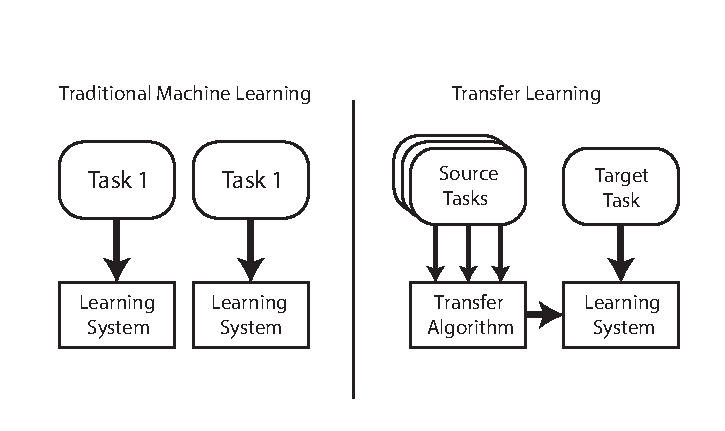
\includegraphics{images/transfervsml.pdf}
    \caption{Transfer Learning vs Traditional ML}
    \label{fig:transfertraditional}
  \end{figure}

  \noindent Transfer learning tries to reduce the learning time of an optimal policy by \textit{reusing} knowledge coming from
  previously solved task (Figure ~\ref{fig:transfertraditional}).\newline



  \section{History and Related Works}
    \noindent Scientific research on transfer learning has attracted more and more attention since 1995.\newline
    Earlier works focus on supervised learning mainly with application in classification and regression problems.
    For example~\cite{liao2005logistic} analyzes the problem of the transfer of knowledge under
    classification settings where the test and training distribution are mismatched. The authors
    propose a solution in which an auxiliary variable $\mu_i$ (for each sample $(\mathbf{x}_i^{a}, y_i^{a})$ in the training dataset)
    is introduced to reflect the mismatch between the two distributions; when $(\mathbf{x}_i^{a}, y_i^{a})$ is too
    different with respect the test distribution an appropriate choice of $\mu_i$ makes the final classifier
    less sensitive to the i$-th$ sample.\newline
    Another example, but applied to regression problems, can be found in~\cite{pardoe2010boosting}; here the authors
    try to develop one of the first general framework for transfer learning and analyze its correctness
    using the \textit{Probably Approximately Correct (PAC)} learning theory. The paper proposes a modification of the classical
    boosting algorithm to successfully include samples coming from a mismatched distribution; the goal is to learn a high
    quality model using as much as possible samples coming from the auxiliary data source.\newline
    A more theoretical work is proposed by~\cite{hanneke2013theory}; the authors explore
    a classification setting in which targets concepts are assumed to be drawn from a known
    distribution. The main goal was to study the total number of sample required to learn all targets to an
    arbitrary specified expected accuracy. The paper shows an interesting connection with the theory of
    active learning that will be discussed in the next chapter.\newline

    \noindent Only in the last 10 years research on transfer learning has focused also on reinforcement learning.
    Works that have been published differ in the type of knowledge transferred (instances, models representation or parameters)
    or in the number and domain of source and target tasks. In this thesis we mainly focus on the transfer of instances
    from a set of source tasks to a single target task; considering this setting some interesting results are presented
    in~\cite{lazaric2008transfer} where the authors successfully show (empirically) that when the samples coming from the
    source tasks are sufficiently \textit{symilar} to ones already collected for the target task, the transfer
    of instances is possible and permits to significantly reduce the time needed to learn an optimal
    policy on the target task.\newline
    A more theory-oriented work appears in~\cite{lazaric2011multiple}, this paper represents one of the
    first attempt to provide a theoretical formalization of the sample-transfer problem, in particular
    the authors provide a series of theoretical bounds for different transfer algorithm showing the potential
    of knowledge transfer in a single-task learning setting.

  \section{Taxonomy}
    \noindent In this section, inspired by~\cite{lazaric2012transfer}, we report a general classification of
    transfer learning based on: the setting, the transferred knowledge and the objective.
    \subsection{Settings}
      \noindent The settings regards the specification of the state-action domain for the tasks involved in
      the transfer. We can have three different cases:
      \begin{itemize}
        \item \textbf{Transfer from a single source task to a target task with fixed domain}. This
        setting (single source and target task) is often referred in literature as \textit{inductive transfer learning}.
        In this particular situation, we assume that both the source and the target task share the same domain, ie.
        the same state-action space. The transfer algorithm might or might not have access to the target task knowledge
        during the transfer. In the case, no knowledge from the task is available the algorithm can only
        perform a very simple transfer (without regarding the problem of the negative transfer) and directly use
        this knowledge in the target task. On the other hand if some knowledge is available from the target
        task than a more complex transfer can happen: the algorithm can adapt the knowledge of the source
        to the knowledge already present in the target, for example by only selecting, in the source task,
        those samples that are likely to be generated by the model of the target task.

        \item \textbf{Transfer across multiple tasks with fixed domain}. In this scenario we assume that many source tasks are
        available. Again, also in this case, all the tasks involved (target and sources) share the same state-action space.
        We expect that, as the number of source task increases, the performance of the target task to be much
        better compared with the previous case.

        \item \textbf{Transfer across multiple tasks with different domains}. This case represents the most general
        situation: multiple tasks are available and each task has a different state-action domain. In this scenario,
        to manage the complexity of the problem, many of the proposed algorithms reduces to the case with a single
        source and target task with different domains and focuses on the problem of defining an efficient mapping
        between the domains of the source and target task.
      \end{itemize}

    \subsection{Knowledge}
      \noindent In every transfer learning algorithm, a central problem is how to define how knowledge is
      actually used to transfer information from the source task to the target task. A possible
      categorization proposed by~\cite{lazaric2012transfer} classify the possible knowledge transfer
      approaches in: instance transfer, representation transfer and parameter transfer:
      \begin{itemize}
        \item \textbf{Instance transfer}. In this scenario, the transferred knowledge assumes the shape of
        samples of trajectories collected in the source tasks. Each sample can be viewed as a tuple
        of four elements: the staring state $s$, the action taken in $a$, the next state $s'$ reached
        after applying $a$ to $s$ and the relevant reward $r$. The transferred samples can now be used
        in the target task, in a model-free approach, for example, to build an accurate approximation
        of the value function of each state.

        \item \textbf{Representation transfer}. The idea is that each RL algorithm uses a specific
        representation of the task and of its solution. After the source tasks have learned an accurate
        solution, the transfer algorithm tries to abstract the different task-solution representations
        to permit the target task to take advantage of them. Examples range from the use of reward
        shaping functions to MDP augmentation through options.

        \item \textbf{Parameter transfer}. Every RL algorithm is characterized by a series of parameters
        that define its own initialization. The key idea is that a good initialization can provide
        a big advantage, in terms of time to convergence, to the RL algorithm running over the target task.
        Examples can be the initial Q values for a Q-Learning algorithm or the learning rate $\alpha$ for a
        more generic algorithm. In some other situation it may be useful to adapt and change the parameters
        according to the target task.
      \end{itemize}

    \subsection{Objectives}
      \noindent It happens often in machine learning (especially in unsupervised settings) to have difficulty
      in measuring the quality of the results. This is true also in transfer learning where several metrics have been defined:
      \begin{itemize}
        \item \textbf{Learning speed improvement}. Here the objective is to measure the gain of the transfer algorithm
        in terms of amount of experience needed to learn the target task. The complexity is then measured in terms
        of samples needed to learn the optimal policy, often referred in literature (especially in supervised learning
        settings) as sample complexity. This type of objective is common when the algorithm is based on the transfer of
        instances. In practice three different metrics are commonly used: \textit{time to threshold}, \textit{area ratio}
        and \textit{finite-sample analysis}. Time to threshold measures how much experience (ie. samples) are needed to
        the algorithm to reach a fixed threshold, the main disadvantage is that the threshold may be arbitrarily chosen
        and bad representing the real situation. The area ratio is formally defined as the ratio between the learning
        curve with and without transfer, precisely:
        \begin{equation*}
          r = \frac{\text{area with transfer} - \text{area without transfer}}{\text{area without transfer}}
        \end{equation*}
        while this metrics does not suffer from the disadvantage previously described, it is scale dependent; that is
        it depends on the unit of measure of the learning curve.\newline
        The last metric represents a more theoretical approach: the idea is to derive bounds that strictly
        depend on the algorithm used, the number of samples available from the source task and the initialization
        parameters of the algorithm itself.

        \item \textbf{Asymptotic improvement}. In the major part of the applications of transfer algorithms, obtaining
        an optimal solution over the target task is often infeasible. In this situation, usually, we are interested
        in getting the solution that asymptotically achieves the best performances.
        This type of objective is usually targeted by representation transfer
        algorithm where the structure of the hypothesis space is transformed so to accurately approximate the solution
        of the target task. Up to date no transfer learning algorithm is guaranteed to improve the average approximation
        error with respect to a non-transfer algorithm.

        \item \textbf{Jumpstart improvement}. This type of objective is usually targeted by parameters transfer
        algorithms. As already mentioned above the performance of any reinforcement learning algorithm strongly
        depends on the initialization of the parameters. A bad initialization often negatively bias the target task
        and leads to longer times of convergence. Common ways to measure this type of improvements are often related
        to the comparison of the performance of the algorithm, in one case initialized with a suitable hypothesis and
        in another randomly initialized.
      \end{itemize}

      \section{Bias-Variance tradeoff}
      	\noindent In this section, we revise the theory behind of the bias-variance tradeoff. This concept represents a key idea in a
      	general machine learning framework and plays a central role in this thesis.
      	For this discussion we do not focus only on the reinforcement learning framework given that this concept is much more general.\newline

      	\noindent The idea behind the bias-variance dilemma is that for any machine learning algorithm the prediction error can
      	always be decomposed in the sum of three components:
      	\begin{equation*}
      		Total Error = Irreducible Error + Bias + Variance
      	\end{equation*}
      	The irreducible error, as the term suggest, can not be reduced regardless the algorithm used. It is the error
      	introduced from the particular realization of the training dataset $\mathcal{D}$, it represents the intrinsic error present in the data.\newline
      	Assume $\mathcal{H}$ to be the space of all the possible concepts (id. functions, also referred as hypothesis) learnable by any machine learning algorithm.
      	Suppose to fix a precise algorithm $\mathcal{A}$ and indicated with $\mathcal{C} \subset \mathcal{H}$ the set of concepts algorithm $\mathcal{A}$ can produce
      	as output. The true model (ie. the concepts that we are trying to learn) $\hat{f}$ might be inside or outside $\mathcal{C}$. On the basis of the samples
      	inside the dataset we can estimate an error function $L$ that, given an hypothesis, it returns the generalization error. We indicate as $\bar{f}$ the
      	concept learnt by $\mathcal{A}$ by minimizing $L$.\newline
      	The situation is summarized by figure~\ref{fig:biasvariance}\newline

      	\noindent The \textbf{bias} can be seen as the distance between the hypothesis learnt by $\mathcal{A}$ and the true concept $\hat{f}$. On the
      	other side the \textbf{variance} can be seen as the difference between what the algorithm has learnt from a particular
      	dataset and what the algorithm expect to learn.\newline
      	Consider the case where we have a perfect estimation of $L$ (ie. when the dataset $\mathcal{D}$ contains an infinite number of samples);
      	in this case we have an extremely low variance while the bias depends wether $\hat{f}$ is inside or outside $\mathcal{C}$.\newline
      	Suppose now that $\mathcal{D}$ contains a limited number of samples, then the estimation of $L$ will not be perfect but it will depend on
      	the number of samples available and on the complexity of $\mathcal{A}$; the higher the complexity of the model and the lower the number of samples
      	the higher the variance (\textit{overfitting}). The smaller the complexity of the model the higher the bias (\textit{underfitting}). The idea is
      	summarized in figure~\ref{fig:biasvariancegraph}.

      	\begin{figure}[!tbp]
      	  \centering
      	  \begin{minipage}[b]{0.4\textwidth}
      	    \includegraphics[scale=0.55]{images/biasvariance.eps}
      	    \caption{The hypothesis space $\mathcal{H}$, the true function $f$ and the error function (color gradient) }
      			\label{fig:biasvariance}
      	  \end{minipage}
      	  \hfill
      	  \begin{minipage}[b]{0.5\textwidth}
      	    \includegraphics[scale=0.55]{images/biasvariancegraph.eps}
      	    \caption{The graph shows the relationship between bias,variance and total error with respect to the model complexity}
      			\label{fig:biasvariancegraph}
      	  \end{minipage}
      	\end{figure}


      	\noindent The \textit{dilemma} consists in managing the complexity of the model, the power of the model and the number of samples in the
      	dataset to reach a situation where both variance and bias are close to zero, that is minimize as much as possible the total error
      	of the model.

      	\noindent As already highlighted the bias-variance dilemma is fundamental importance also in the context of transfer learning.
      	When samples are transferred from a source task to a target task we are introducing a bias in the learning performance
      	of the target, but at the same time, given that more samples are available for the learning algorithm, we are reducing
      	the variance of the estimation. The objective of the next chapters will be to seek the optimal tradeoff between the
      	bias increase and variance reduction.

        \section{Formal specification and Assumptions}
          \noindent In the following we provide the notation used in the rest of the work.
          \begin{definition}
            A task $T$ is an MDP defined as a tuple $(\mathcal{S},\mathcal{A},\mathcal{P}_T,\mathcal{R}_T,\gamma)$.
          \end{definition}

          \noindent In our situation we have a set of source MDPs plus a target MDP: $\mathcal{M}_1,\mathcal{M}_2, \dots, \mathcal{M}_n$
          where $\mathcal{M}_1, \dots, \mathcal{M}_{n-1}$ are the source MDPs and $\mathcal{M}_n$ is the target MDP.\newline
          In our framework we focus on the transfer of samples between the source MDPs and the target MDP; a
          sample in our context is a tuple $(s,a,s^{'},r)$ where $s$ and $s^{'}$ are states, $a$ is an action and $r$ is the reward associated with the transition $s,a,s'$.\newline
          We also assume that all the tasks (target included) share the same state-action space, so that no mappings are needed
          to transfer the samples.\newline

          \noindent Precisely we suppose that a number $N_t$ of samples are available
          from the target task and $N_s$ total samples are available from all the target task, with $N_t << N_s$.\newline
          Moreover, as already stated, a transfer algorithm cannot blindly transfer all the samples to the target
          task due to the possibility of a negative transfer; indeed samples coming from the target task bring a certain
          amount of variance reduction and are unbiased while samples coming from the source tasks still bring to a reduction
          over the variance but they are biased given that they come from a task that a priori might be very different
          from the target task. Therefore when transferring samples from the source tasks an estimation of the bias must be available
          and more precisely we say that the transfer is positive when the increment of the bias is lower than the decrement of the variance.
          In our case we provide a way to minimize the bias introduced by the transferred samples.

  %\input{chapters/chapter4}
  \chapter{Weighted Fitted Q-Iteration}
  \vspace{2cm}

  \lettrine[lines=2]{I}n this chapter we introduce the central algorithm of this thesis: Weighted Fitted Q-Iteration (from now on abbreviated as WFQI from now on).\newline
  The WFQI algorithm is a \textit{batch-mode} reinforcement learning algorithm which, as the FQI algorithm described in Chapter 2, try to build
  an approximation of the Q-function of the MDP by iteratively extending the optimization horizon.\newline
  WFQI is built on top of FQI, it maintains all the properties described in the previous chapters but it also uses
  the additional information in the dataset to permit the transfer of experience sample.\newline
  Again it is a batch-mode learning algorithm so the learning procedure is divided into two distinct parts: in the first part
  samples are collected, according to some policy, only from the target task. In the second part the samples in the dataset
  are actually used to approximate the Q-function.\newline
  One important difference with respect to the standard FQI algorithm consists in the information required: each sample
  must contain additional information to permit its transfer. The overall transfer procedure, in conjunction with
  importance sampling, is depicted in figure \ref{transferwfqi}.

  \noindent Another important property, inherited from FQI, is the use of a regression algorithm in the learning phase of the algorithm
  Again this simple idea permits WFQI to take advantage of the specific regression algorithm.
  Moreover our \textit{weighed} approach to the problem of transfer, being it totally separate from weight calculation procedure,
  permits a very high flexibility in the transfer process. Ideally, we could select the weights that perfectly minimizes the effect
  of the negative transfer. In general, depending on the specific problem, many others choices are possible.\newline

  \noindent A key point in our approach is the use of weights along with the samples in the datasets. These weights
  are defined according to idea behind \textit{importance sampling}.\newline
  In many applications, we face the problem of estimating the mean of a random variable $\mu = \mathrm{E}[f(\pmb{X})]$
  where the function $f(x)$ is always 0 except for a small region $R$ and the probability for $\pmb{X}$ to
  assumes values in $R$, $\mathbb{P}(\pmb{X} \in R)$, is very small.\newline
  In such situation the application of stochastic methods, like Monte Carlo, fails because it is very difficult to have
  even one point inside the interesting region $R$. Problems of this type arise very often in practice and in very
  different domains such as physics, bayesian inference, rare events simulations etc.\newline
  The central point is that to effectively apply Monte Carlo-like techniques some points from the interesting (important)
  region must somehow be taken. The idea of importance sampling is to take samples not from the original distribution
  of $\pmb{X}$ but from an auxiliary distribution, known as the \textit{importance distribution}, that overweights the important
  region, hence the name \textit{importance} sampling.\newline
  \noindent The use of importance sampling can bring huge gains and make tractable problems where Monte Carlo is
  usually ineffective. On the other hand there are also known situation where the use of an importance distribution
  in place of the nominal one can be a disadvantage yielding estimates with extremely high variance (in some case infinite).\newline

  \noindent The first part of this chapter is dedicated to the description and motivation of WFQI, while the remaining is
  devoted to the problem of the weights estimation.

  \vspace{3cm}
  \section{The WFQI Algorithm}
    \noindent In this section we describe WFQI and we analyze its properties and relationship with respect to FQI.
    Notice that, being the weight estimation problem totally separated from WFQI, in this section we describe
    WFQI assuming that the weights for each sample are known.

    \begin{figure}
      \centering
      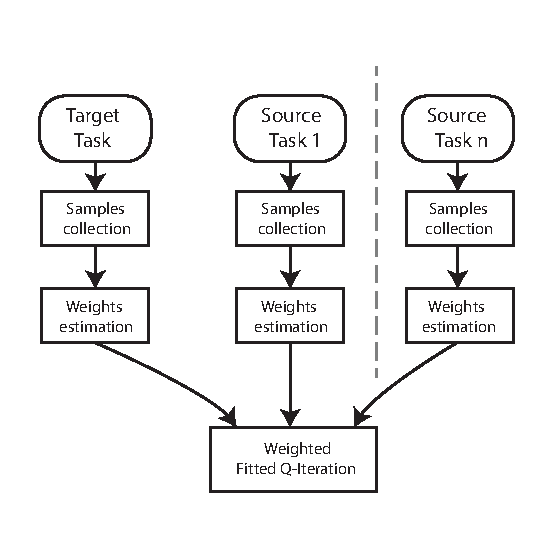
\includegraphics[scale=1.2]{images/transferwfqi.pdf}
      \caption{The overall process of transfer: from the collection to the use with WFQI}
      \label{transferwfqi}
    \end{figure}
    \noindent Algorithm \ref{fittedqw} describes a pseudocode version of Weighted Fitted Q-Iteration.

    \begin{algorithm}[H]
        \caption{Weighted Fitted Q-Iteration algorithm}\label{fittedqw}
        \begin{algorithmic}[1]
          \Procedure{WFQI($\mathcal{D} = (s,a,s',r,w_s,w_r)_{k=1}^{N}, myWeightedRegressionAlg$)}{}
            \State $k \gets 0$
            \State $\hat{Q}^{0}(s,a) \gets 0$ $\forall (s,a) \in S \times A$
            \State $D' \gets (s_k,a_k,r_k)_{k=1}^{N}$
            \State $\hat{Q}^{1} \gets myWeightedRegressionAlg(\mathcal{D}', w_r)$

            \State $\mathcal{D}' = \emptyset$
            \While {$checkStoppingCriteria()$}
              \State $k \gets k + 1$
              \For {$l = 1$ $\text{to}$ $N$}
                \State $i_l = (s_l, a_l)$
                \State $o_l = Q^{1} + \gamma \max_{a' \in A} \hat{Q}_{k-1}(s',a')$
                \State $\mathcal{D}' \text{+=}$ $(i_l,o_l)$
              \EndFor
              \State $\hat{Q}^{k} \gets myWeightedRegressionAlg(\mathcal{D}', w_s)$
            \EndWhile
          \EndProcedure
        \end{algorithmic}
    \end{algorithm}

    \noindent More informations about the specific implementation of WFQI are given in appendix A.\newline

    \noindent The main differences with respect to the standard FQI algorithm are:
    \begin{itemize}
      \item \textbf{Dataset}: The experience sample contained in the dataset are enhanced with additional
        information namely $w_r$ and $w_s$. These informations are needed by WFQI in order to permit
        the transfer of samples coming from different source tasks. These weights, for reward ($w_r$) and
        transition model ($w_p$), need to be separately estimated and then injected inside the
        existing dataset.

      \item \textbf{Regression Algorithm}: The only real modification needed in algorithm \ref{fittedqw},
        with respect to the standard FQI, consists in a new requirement over the used
        regression algorithm: in order to effective transfer samples, the regression
        algorithm must permit to specify, for each sample, a weight and accordingly use
        it in the fitting procedure. Notice that different weights are used in different
        part of the algorithm; at the iteration 0 the Q-function is initialized to zero
        this means that the initial dataset is exclusively built using the rewards of the
        sample thus making useless the use of $w_s$. Moreover, in the successive iterations,
        instead of building the dataset $\mathcal{D}'$ using the usual Bellman equation
        $o_l = r + \gamma \max_{a' \in A} \hat{Q}^{k-1}(s',a')$ we substitute $r$ with $\hat{Q}^{1}$
        which represents the weighted reward function (according to $w_r$), thus, in the regression
        we only need to weight the samples with $w_s$.
    \end{itemize}

  \section{Algorithm Motivation}
    \noindent The motivation of using Importance Sampling in the framework of Transfer Learning comes directly
    from the need of a strong theoretical basis behind the transfer procedure. Many sample-based transfer approaches,
    see for example \cite{lazaric2008transfer}, focus on defining measures to capture the concept of similarity
    between tasks and samples. In our case, the possibility to support the calculation and use of each weight
    with a strong theoretical background gives the possibility, not only to perform an effective transfer of samples,
    but also to quantify and control the amount of bias introduced in the estimation.\newline

    \noindent WFQI exploits the same idea of the standard FQI algorithm. It uses a dataset of experience
    sample, previously collected, in conjunction with a generic weighted regression algorithm to produce an estimation
    of the Q-function for the target task. The main difference, as already outlined above, is that it permits
    the use of samples coming from tasks different from the one it tries to solve.\newline
    If we assume that $w_p$, $w_r$ are the \textit{ideal} weights (ie. given by an oracle),
    then, according to the results of importance sampling presented in the previous chapter, the use of
    the corresponding samples coming from the set of source tasks is unbiased and may lead to a potential
    reduction in the variance of the estimation.\newline
    On the other side, the ideal weights can not be calculated in practice given that their knowledge would
    require a perfect knowledge of the reward and transition model of the target task meaning that nothing has to
    be learned. When using the estimated weights the use of the corresponding samples from the set of source tasks in
    the learning process of the target is not unbiased. This means that in addition to the potential reduction in
    variance an additional increase in bias is possible.\newline
    The necessity of calculating the pair of weights for each source sample motivates the need of explicitly modelling
    the reward and transition model for all the tasks involved in the transfer (this problem will be addressed in the
    final part of this chapter).

    \noindent Another important characteristic of WFQI is the peculiar use of the weights associated with each
    samples, that permits to transfer samples even in situations where either the reward or the dynamics
    represented by the sample is significantly different from the target task.
    \noindent A formal and detailed theoretical analysis of the errors coming from the use of estimated weights
    is provided in the last sections of this Chapter.\newline

    \noindent In conclusion WFQI represents a very simple and intuitive modification of
    the original FQI algorithm. Besides, these adjustments do not negatively affect the computational
    complexity of the algorithm (only two additional multiplication per iteration are needed) and
    has the remarkable advantage of permitting the reuse of past knowledge (which in general tends to speed-up the learning process).\newline
    It also important to note some of the possible disadvantages: WFQI uses extensively the underlying idea
    of importance sampling and therefore may not be effective in every situation.

\section{Introduction to Importance Sampling}
  \noindent In this section, and in the remaining part of this Chapter, we introduce the general theory of Importance Sampling (sometimes abbreviated as IS), we start from a problem apparently
  unrelated with the problem of transfer in RL, later we describe how the transfer of samples across tasks can be reframed into
  the general idea of IS.\newline

  \noindent Let $\pmb{X}$ be a continuous random variable distributed according to a density function $p(x)$. Our problem is to find:
  \begin{equation}
    \mu = \mathrm{E}[f(\pmb{X})] = \int_{\mathcal{R}} f(\pmb{x})p(\pmb{x}) d\pmb{x}
    \label{mean1}
  \end{equation}
  \noindent where $p$ is a probability density function over $\mathcal{R} \subseteq \mathbb{R}^{d}$ and $f$ is a
  generic function over $\pmb{X}$. $p$ is known as the \textbf{nominal distribution}.\newline
  As already stated we want to estimate the mean of $f(\pmb{X})$ not from samples drawn from $p$ but from a set
  of samples drawn from an auxiliary distribution $q$ from now on known as the \textbf{importance distribution}.
  Recalling equation \ref{mean1} we have with simple algebraic manipulation:
  \begin{equation*}
    \mu = \int_{\mathcal{R}} f(\pmb{x})p(\pmb{x}) d\pmb{x} = \int_{\mathcal{R}} f(\pmb{x}) \frac{p(\pmb{x}) q(\pmb{x})}{q(\pmb{x})} d\pmb{x} =
     \mathbb{E}_{q} \left [f(\pmb{X})\frac{p(\pmb{X})}{q(\pmb{X})} \right ]
  \end{equation*}
  $w(\pmb{x}) = \frac{p(\pmb{x})}{q(\pmb{x})}$ is the \textbf{importance weight} for the sample $\pmb{x}$. The result
  is very intuitive: we can estimate the mean of $f(\pmb{X})$ by drawing samples from $q$ and correcting them
  with a multiplicative factor equal to $\frac{p(\pmb{X})}{q(\pmb{X})}$.\newline

  \noindent Notice that the probability density function $q(x)$ does not to be strictly positive everywhere but it sufficient
  to have $q(x) > 0$ whenever $f(x)p(x) \neq 0$. It is also important to notice that $q(x)$ can never be equal to 0
  (if a sample has been drawn from $q$ then $q(x) > 0$ in any case).\newline

  \noindent We now proceed to give some additional definition and we state some results to understand when the use of importance sampling
  is useful and when it is not.\newline
  We define the importance sampling \textit{estimate}, $\hat{\mu}_q$, of $\mu$ as
  \begin{equation}
    \hat{\mu}_q = \frac{1}{N} \sum_{i=1}^{N} \frac{f(X_i)p(X_i)}{q(X_i)}
    \label{meanestimate}
  \end{equation}

  \noindent The fundamental point is that we are able to compute the estimate in \ref{meanestimate} only when both $p$ and $q$ are known.
  This is not always the case, in particular when we will try to apply these ideas to the problem of the transfer of knowledge
  we will need to resort to some method to estimate the ration between the two densities. For this section we will assume that
  the ration $p/q$ is computable.

  \begin{theorem}[\cite{importance2013Owen}]
    Let $\hat{\mu}_q$ the estimate provided by equation \ref{meanestimate} where $\mu = \int_{\mathcal{D}} f(\pmb{x})p(\pmb{x}) d\pmb{x}$
    and $q(\pmb{x}) > 0$ whenever $f(\pmb{x})p(\pmb{x}) \neq 0$. Then $\mathbb{E}_{q}[\hat{\mu}_q] = \mu$ and $\text{Var}_{q}[\hat{\mu}_q] = \frac{\sigma^{2}_{q}}{N}$
    where
    \begin{equation}
       \sigma^{2}_{q} = \int_{\mathcal{D}} \frac{(f(\pmb{x}) p(\pmb{x}))^2}{q(\pmb{x})} d\pmb{x} - \mu^{2} = \int_{\mathcal{D}} \frac{(f(\pmb{x}) p(\pmb{x}) - \mu q(\pmb{x}))^{2}}{q(\pmb{x})} d\pmb{x}
       \label{theorem2}
    \end{equation}
  \end{theorem}
  \begin{proof}
    Let $\mathcal{Q} = \{\pmb{x} | q(\pmb{x}) > 0\}$ then
    \begin{equation*}
      \begin{multlined}
        \mathbb{E}_{q} \left [ \frac{f(\pmb{X})p(\pmb{X})}{q(\pmb{X})} \right ] = \int_{\mathcal{Q}} \frac{f(\pmb{x})p(\pmb{x})}{q(\pmb{x})} q(\pmb{x}) d\pmb{x} = \int_{\mathcal{Q}} f(\pmb{x}) p(\pmb{x}) d\pmb{x} = \\
        \int_{\mathcal{D}} f(\pmb{x}) p(\pmb{x}) d\pmb{x} + \int_{\mathcal{Q} \cap \mathcal{D}^{c}} f(\pmb{x}) p(\pmb{x}) d\pmb{x} - \int_{\mathcal{D} \cap \mathcal{Q}^{c}} f(\pmb{x}) p(\pmb{x}) d\pmb{x} = \\
        \int_{\mathcal{D}} f(\pmb{x}) p(\pmb{x}) d\pmb{x} = \mu = \mathbb{E}_{q}[\hat{\mu}_q]
      \end{multlined}
    \end{equation*}

    \noindent The second part of the proof can be obtained in a similar way:
    \begin{equation*}
      \text{Var}[\hat{\mu}_{q}] = \frac{1}{n} \left [ \int_{\mathcal{Q}} \left ( \frac{f(\pmb{x})p(\pmb{x})}{q(\pmb{x})} \right )^{2} q(\pmb{x}) d\pmb{x} - \mu^{2} \right ] =
        \frac{1}{n} \left [ \int_{\mathcal{D}} \left ( \frac{f(\pmb{x})p(\pmb{x})}{q(\pmb{x})} \right )^{2} q(\pmb{x}) d\pmb{x} - \mu^{2} \right ]
    \end{equation*}

    \noindent Simple manipulations gives equation \ref{theorem2}.
  \end{proof}

  \noindent Expressions in equation \ref{theorem2} give a simple way to understand when importance sampling can succeed or fail.
  The best importance distribution is the one that minimizes $\int_{\mathcal{D}} \frac{(f(\pmb{x}) p(\pmb{x}))^2}{q(\pmb{x})} d\pmb{x}$.
  Moreover if we analyze the right integral expression (always in \ref{theorem2}) it is easy to notice that the numerator is small
  when $f(\pmb{x})p(\pmb{x})$ is similar to $\mu q(\pmb{x})$. This happens when $f(\pmb{x})p(\pmb{x})$ is proportional to $q(\pmb{x})$.
  On the other hand also the denominator can cause some problems: a region with a small $q$ can amplify whatever lack of proportionality
  in the numerator.\newline
  In theory choice of $q$ such that $\sigma^{2}_{q} = 0$ are possible but of course of no use in practice. The choice
  of a good importance distribution is a complex problem that requires educated guesses, numerical search and domain-specific knowledge.


\section{Transfer with Importance Sampling}

\noindent In this section we face the problem of the transfer of knowledge across multiple tasks. We assume the context of
batch-mode reinforcement learning and, for the sake of simplicity, we suppose that a single source task is available. Later on
we will extend our transfer model for the case of multiple source tasks.\newline
We suppose some samples have been previously collected from the target task producing a dataset $\mathcal{T} = \{(s_{i},a_{i},s'_{i},r_{i})\}_{i=1}^{N_t} $ and
similarly some samples (the samples that have to be transferred) have been obtained from the source task producing a dataset $\mathcal{S} = \{(s_{i},a_{i},s'_{i},r_{i}) \}_{i=1}^{N_s}$.
Typically we will assume $N_t << N_s$.\newline

\subsection{Single Source Task}
  \noindent Suppose to transfer a sample $(s_{i}, a_{i}, s'_{i}, r_{i})$ from the source task to the target task. The transfer
  affects the target task on two sides: the reward model and the probability transition model. \newline
  Suppose, for simplicity, to consider only the effect on the reward. This last element is modeled as a function:
  \begin{equation}
    r: S \times A \rightarrow \mathbb{R}
  \end{equation}
  \noindent Given a state-action pair the function will return the expected reward for the agent. Every time a transfer
  is performed we are introducing a bias inside the estimation of the reward function for the target task.\newline
  The idea is to apply importance sampling to the samples of the source task used in the estimation of the reward function
  of the target task. Let be $w_r$ the likelihood weight associated to the reward model. Select a sample pair $(s,a,s',r)$ from
  the source task (we are assuming that the source and target share the same state-action space). Then we have
  \begin{equation}
    w_{r} = \frac{\text{likelihood of $r$ to be generated in }\mathcal{S}}{\text{likelihood of $r$ to be generate in }\mathcal{T}}
  \end{equation}

  \noindent There are some important facts to be observed:
  \begin{itemize}
    \item When the stochastic model of the reward is perfectly known in both task
      the $w_r$ can be perfectly calculated, in this setting the use of $r$ in the
      target is completely unbiased. Of course if the two tasks are quite different
      then the reduction of variance carried by $r$ will be much lower with respect to
      the case where $r$ is directly sampled from the target.

    \item In practice the reward model of the source and target tasks are not known
      (otherwise the agent has nothing to learn, at least for the reward, and transfer will
      be useless). This means that we need a procedure to accurately estimates the likelihood
      for both tasks. A possible procedure will be discussed in the next section.

    \item As already observed in the general discussion about importance sampling, the
      denominator of $w_r$ can never be zero (if the sample has been drawn from the source
      then its likelihood is by definition different from 0). Some numerical problems may arise
      when the denominator is close to zero, in such cases $w_r$ may be very large and this
      tends to increase the variance of the estimation.
  \end{itemize}

  \noindent Identical considerations hold for the probability transition model, also in this case we have
  a stochastic model that given a state-action pair returns a probability distribution over the next state.\newline
  Again the idea is to apply importance sampling also to the transition model, this means that a second
  likelihood weight $w_p$ must be defined. Fix a sample $(s,a,s',r)$ to be transferred then:
  \begin{equation}
      w_{p} = \frac{\text{likelihood of $s \rightarrow s'$ to be generated in }\mathcal{S}}{\text{likelihood of $s \rightarrow s'$ to be generate in }\mathcal{T}}
  \end{equation}

  \noindent The overall transfer procedure for the single source case requires to collect the two datasets $\mathcal{T}$ and $\mathcal{S}$ from
  the two tasks. A weight estimation procedure is applied to the datasets. The output is a new pair of datasets $\mathcal{S}'$ and $\mathcal{T}'$ where
  \begin{equation*}
    \begin{cases}
      \mathcal{S}' = \{ (s_{i},a_{i},s_{i}',r_{i},w_{r}^{i},w_{p}^{i}) \}_{i=1}^{N_s} \\
      \mathcal{T}' = \{ (s_{i},a_{i},s_{i}',r_{i},1,1) \}_{i=1}^{N_t}
    \end{cases}
  \end{equation*}
  Notice that the weights for the samples coming from the target tasks (that do not need to be transferred) are
  obviously fixed to 1.

\subsection{Multiple Source Tasks}
  \noindent The extension to the case where multiple source tasks are present is straightforward. Let $\mathcal{T}$ the dataset of the samples
  collected from the target task and let $\mathcal{S}_i$ the dataset of samples collected from the $i$-th source task.\newline
  Then the transfer procedure works exactly as in the single source case: the source datasets are considered one at a time,
  a weight estimation procedure is applied to the samples contained in the current dataset so that we obtain
  \begin{equation*}
    \mathcal{S}_{i} = \{ (s_{i}^{j}, a_{i}^{j}, s_{i}^{'j}, r_{i}^{j}, w_{r}^{i,j}, w_{p}^{i,j}) \}_{j=1}^{N_{s}}
  \end{equation*}
  This is repeated for every source tasks. As in the previous case for the target task the weights for reward and
  transition model are fixed to 1 (ie. nothing to transfer).\newline

  \noindent Two remaining open problems are:
  \begin{enumerate}
    \item How to estimates the likelihood weights for transition and reward model when the relevant densities are not known? This
    problem will be addressed in the next two sections.
    \item How to effectively use the likelihood weights inside a learning algorithm? The conclusive sections of this chapter will propose a variation
    of the well-known FQI algorithm to include the information coming from the likelihood weights.
  \end{enumerate}

\subsection{Transfer of Samples vs Transfer of Trajectories}
  \begin{figure}
    \centering
    \includegraphics{images/trajectorysample.eps}
    \caption{Trajectory vs Sample}
    \label{trajectorysample}
  \end{figure}

  \noindent One implicit assumption done so far is the type of knowledge to be transferred to the target task.
  In the last years two main approaches have been proposed: the transfer of \textit{trajectories} or the transfer
  of \textit{samples}. Figure \ref{trajectorysample} depicts the difference between the two entities.\newline
  A trajectory is characterized by an initial state, a terminal state (where the trajectory ends because either
  one of the goal state or a maximum horizon has been reached by the agent) and by a series of intermediate states
  that link the initial with the terminal state. Each state is linked with each other with an action that performs
  the transition between the two states. On the other hand, a sample is characterized by four-tuples $(s,a,s',r)$
  where $s$ is the state in which the agent is performing action $a$ reaching the successive state $s'$ and
  obtaining reward $r$.\newline

  \noindent The transfer of a sample is, in our specific transfer learning framework, more advantageous
  than the transfer of an entire trajectory. Indeed the transfer of an entire trajectory does not
  permit to decide which part of the trajectory is actually beneficial for the transfer and which are not.
  There may be part of the trajectory that could represents dynamics that may negatively bias the agent
  inside the target task.\newline
  On the other hand, the transfer of samples permits a finer control over the transfer process.
  Once the samples are collected from the source tasks we loose the information about the specific
  trajectory each sample belongs to. Our approach permits to estimate a pair of weights for each sample,
  these weights are used by the learning algorithm to correct the bias introduced by such samples.\newline

  \noindent As an example consider the problem of the transfer of a trajectory where 99 \% of the
  transition/rewards are identical as in the target task but 1 \% of the trajectory is completely
  different with respect the target the target. In this case, the overall likelihood of the trajectory
  will be approximately zero leading to an ineffective transfer. In the case we had considered each
  single sample of the trajectory a much more effective transfer could have been accomplished.

\subsection{Weights Selection}
  \noindent One key point in our transfer procedure is the calculation of the likelihood weights that are used by the
  learning to correct the negative bias. To each sample we associate a pair of weights $w_r$ and $w_p$.
  Given a sample $(s,a,s',r)$ the weight $w_r$ is defined as the ratio between the likelihood of reward $r$
  to be generated in the target task and the likelihood of $r$ to be generated in the corresponding source task
  (from which the sample has been collected). On the other side $w_p$ is the weight associated with the
  transition model and it is defined as the ratio between the likelihood for the transition $s \rightarrow s'$ to
  be generated in the target task and the likelihood, for the same transition, to generated in the correspondent source
  task.\newline

  \subsubsection{Ideal case}
    \noindent In the case where the probabilistic models for reward and transition are perfectly known it
    is possible to calculate the true values for the importance weights of each sample in the dataset.
    We assume that both reward and transition are normally distributed:
    \begin{equation}
      x_{S} \sim \mathcal{N}(\mu_{S}, \sigma^{2}), \quad x_{T} \sim \mathcal{N}(\mu_{T}, \sigma^{2})
    \end{equation}
    where $x$ is either the reward $r$ or the next state $s'$ for a sample $(s,a,x)$.\newline
    In this case the corresponding weight can be obtained applying the definition of importance weight:
    \begin{equation}
      w(x) = exp \left ( -\frac{(x-\mu_{T})^{2}}{2\sigma^{2}} \right ) exp \left ( \frac{(x-\mu_{S})^{2}}{2\sigma^{2}} \right )
      \label{ideal-weights-expr}
    \end{equation}
    Notice that we assume the variance of the reward/transition model to be identical in both the source and target task.
    This assumption is without loss of generality, indeed in the case of different variances we just need to
    consider an additional constant term, $\frac{\sigma^{2}_{S}}{\sigma^{2}_{T}}$, in Equation \ref{ideal-weights-expr}.
    This assumption will be maintained in the next chapters and sections.

  \subsubsection{Non-Ideal case}
    \noindent As already observed in the previous chapters it is not possible, in practice, to perfectly calculate
    the pair of weights for each sample in the dataset. This is due to the fact that the model for the reward and
    transitions are not known in both the source and target task. In the case they were known then we are no more
    in the settings of reinforcement learning but we are solving a dynamic programming problem where the model
    of the environment is perfectly known to the agent and the objective is to approximate the optimal policy.
    In the following, we propose a procedure to estimate the weights based on Gaussian Process (GP) regression.\newline
    The main idea behind the estimation procedure is to make a hypothesis over the reward and
    transition model. Suppose for now to consider only the estimation of the weight associated with the reward, $w_r$.
    We hypothesize a gaussian model for the reward model for both the source and target task. The idea is to place two distinct GP regressors, one for each task,
    over the entire state-action space. For an extensive discussion about GPs refer to appendix B.\newline
    Once the gaussian process has been fitted using the samples in the dataset for the source and target task, we fix
    a sample $(s,a,s',r)$ and we ask a prediction, for the pair $(s,a)$, to the GP associated with the source and to
    the GP associated with the target.\newline
    Now, we proceed to give an extensive description of the estimating procedures.

    \begin{figure}
      \centering
      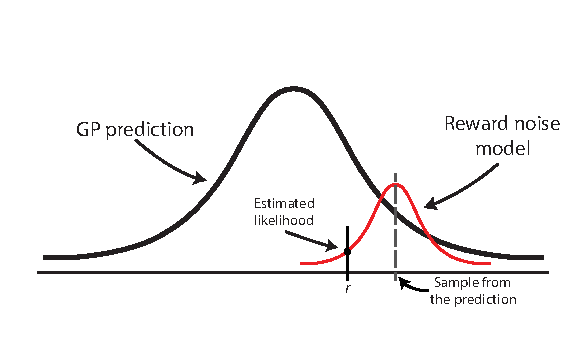
\includegraphics[scale=1.1]{images/gaussian.pdf}
      \caption{Estimating the reward/transition weight from a GP prediction.}
      \label{gaussians}
    \end{figure}

    \noindent A \textit{first} idea to obtain an estimation $\tilde{w}_{x}$ is to directly sample the weights distribution, which
    is unknown and not available in practice.\newline
    Suppose to have a source sample $(s,a,x)$, where $x$ is either $r$ or $s'$, and we want to compute
    its importance weight. First, we predict the distribution if the mean of $x$ under the target model and the
    source model using our previously fitted Gaussian Processes:
    \begin{equation}
      \tilde{\mu}_{T} \sim \mathcal{N}(\mu_{GP,T}, \sigma_{GP,T}^{2}), \quad \tilde{\mu}_{S} \sim \mathcal{N}(\mu_{GP,S}, \sigma_{GP,S}^{2})
      \label{distributions}
    \end{equation}
    Then we consider the estimated importance weights:
    \begin{equation}
      \tilde{w}(x) = \tilde{w}_{x}(\tilde{\mu}_{T}, \tilde{\mu}_{S}) = exp \left ( -\frac{(x-\tilde{\mu}_{T})^{2}}{2\sigma^{2}} \right ) exp \left ( \frac{(x-\tilde{\mu}_{S})^{2}}{2\sigma^{2}} \right )
    \end{equation}
    where the notation $\tilde{w}_{x}(\tilde{\mu}_{T})$ is used to emphasize the dependence on the two means (which now
    are random variables) and on the fixed value of $x$.\newline
    We sample $N_{smp}$ from both $\tilde{\mu}_{T}$ and $\tilde{\mu}_{S}$ then for the $i$-th sample $\mu_{x}^{i}$ we consider the
    two distributions:
    \begin{equation}
      n_{x}^{i} \sim \mathcal{N}(\mu_{x}^{i}, \sigma^{2}_{GP,T}), \quad d_{x}^{i} \sim \mathcal{N}(\mu_{x}^{i},\sigma^{2}_{GP,S})
    \end{equation}

    Then the estimation according to the $i$-th sample is given by:
    \begin{equation}
      w^{i}(x) = \frac{n^{i}(x)}{d^{i}(x)}
    \end{equation}
    Notice that when the prediction from the GP of source and target task are perfect, ie. $\sigma_{GP,T}^{2} = \sigma_{GP,S}^{2} = 0$,
    $\tilde{w}(x)$ converges to $w(x)$.
    The procedure is graphically summarized in Figure \ref{gaussians}.\newline
    Despite being a very simple approach some problems may arise when choosing the final weight among the $N_{smp}$ estimations.
    The selection of different quantiles of the weight distribution may lead, in practice, to very different performance (good in some cases, poor in others). Furthermore
    we do not have any theoretical backup to support the choice of a particular sample among the $N_{smp}$.\newline
    We are able to prove the following result on $\tilde{w}_{x}$:
    \begin{lemma}
      The expectation of $\tilde{w}_{x}(\tilde{\mu}_{T}, \tilde{\mu}_{S})$ under the distributions defined in
      Equation \ref{distributions} is:
      \begin{equation}
        \mathbb{E}[\tilde{w}_{x}(\tilde{\mu}_{T}, \tilde{\mu}_{S})] =
        \begin{cases}
          \frac{\sigma^{2}}{\sigma^{2} - \sigma^{2}_{GP,S}} \frac{\mathcal{N}(x; \mu_{GP,T}, \sigma^{2} + \sigma^{2}_{GP,T})}{\mathcal{N}(x; \mu_{GP,T}, \sigma^{2} - \sigma^{2}_{GP,S})} \quad \sigma^{2}_{GP,S} < \sigma^{2} \\
          \infty \quad Otherwise
        \end{cases}
        \label{mean-weight}
      \end{equation}
    \end{lemma}
    \begin{proof}
      Suppose that $\sigma^{2}_{GP,S} < \sigma^{2}$. Then:
      \begin{equation}
        \begin{aligned}
          & \mathbb{E}[\tilde{w}_{x}(\tilde{\mu}_{T}, \tilde{\mu}_{S})] = \iint \frac{exp \left ( -\frac{(x-\tilde{\mu}_{T})^{2}}{2\sigma^{2}} \right )}{\sqrt{2\pi\sigma^{2}}} \frac{\sqrt{2\pi\sigma^{2}}}{exp \left ( -\frac{(x-\tilde{\mu}_{S})^{2}}{2\sigma^{2}} \right )} \\
          & \frac{exp \left ( -\frac{(\tilde{\mu}_{T}-\mu_{GP,T})^{2}}{2\sigma^{2}_{GP,T}} \right )}{\sqrt{2\pi\sigma^{2}_{GP,T}}} \frac{exp \left ( -\frac{(\tilde{\mu}_{S}-\mu_{GP,S})^{2}}{2\sigma^{2}_{GP,S}} \right )}{\sqrt{2\pi\sigma^{2}_{GP,S}}} d\tilde{\mu}_{T}\tilde{\mu}_{S} \\
          & = \int \frac{exp \left ( -\frac{(x-\tilde{\mu}_{T})^{2}}{2\sigma^{2}} \right )}{\sqrt{2\pi\sigma^{2}}} \frac{exp \left ( -\frac{(\tilde{\mu}_{T}-\mu_{GP,T})^{2}}{2\sigma^{2}_{GP,T}} \right )}{\sqrt{2\pi\sigma^{2}_{GP,T}}} d\tilde{\mu}_{T} \\
          & \int \frac{\sqrt{2\pi\sigma^{2}}}{exp \left ( -\frac{(x-\tilde{\mu}_{S})^{2}}{2\sigma^{2}} \right )} \frac{exp \left ( -\frac{(\tilde{\mu}_{S}-\mu_{GP,S})^{2}}{2\sigma^{2}_{GP,S}} \right )}{\sqrt{2\pi\sigma^{2}_{GP,S}}} d\tilde{\mu}_{S}
        \end{aligned}
      \end{equation}

      \noindent The first integrand is over the product of two Gaussian densities, which is known to be (see \cite{bromiley2003products}):
      \begin{equation}
        \mathcal{N}(\tilde{\mu}_{T}; \bar{\mu}_{T}, \bar{\sigma}^{2}_{T}) \mathcal{N} (x; \mu_{GP,T}, \sigma^{2}+\sigma_{GP,T}^{2})
      \end{equation}
      where the values of the mean $\bar{\mu_{T}}$ and variance $\bar{\sigma}^{2}_{T}$ of the first density are not important
      to complete the proof since such density integrates out in the previous equation. By adopting a  procedure as the
      one described in \cite{bromiley2003products}, we can write the ratio of the two Gaussians densities in the second integral
      as:
      \begin{equation}
        \frac{\sigma^{2}}{\sigma^{2}-\sigma^{2}_{GP,S}} \frac{\mathcal{N}(\tilde{\mu}_{S}; \bar{\mu}_{S}, \bar{\sigma}^{2}_{S})}{\mathcal{N}(x; \mu_{GP,S}, \sigma^{2}-\sigma^{2}_{GP,S})}
      \end{equation}
      \begin{proof}
        It can be easily verified by taking:
        \begin{equation}
          \bar{\mu}_{S} = \frac{\tilde{\mu}_{S} - \tilde{\mu}_{GP,S}}{\sigma^{2} - \sigma^{2}_{GP,S}}, \quad \bar{\sigma}^{2} = \frac{\sigma^{2}\sigma^{2}_{GP,S}}{\sigma^{2}-\sigma_{GP,S}^{2}}
        \end{equation}
        Then by substituting and writing explicitly the Gaussian densities we have:
        \begin{equation*}
          \begin{aligned}
            & \frac{\sigma^2}{\sigma^{2}-\sigma^{2}}\frac{\sqrt{2\pi}}{\sqrt{2\pi}}\frac{\sqrt{\sigma^{2}-\sigma_{GP,S}^{2}}} {\sqrt{\frac{\sigma^{2}\sigma^{2}_{GP,S}}{\sigma^{2}-\sigma^{2}_{GP,S}} }} \exp \left ( \frac{(x-\mu_{GP,S})^{2}}{2(\sigma^{2}-\sigma^{2}_{GP,S})} \right )
              \exp \left ( -\frac{(\tilde{\mu}_{S} - \bar{\mu}_{S})^{2}}{2 \frac{\sigma^{2}\sigma^{2}_{GP,S}}{\sigma^{2}-\sigma^{2}_{GP,S}}} \right ) = \\
            & \frac{\sigma}{\sigma_{GP,S}} \exp \left ( \frac{\sigma^{2}_{GP,S}x^{2} + \sigma^{2}_{GP,S}\tilde{\mu}^{2}_{S} - 2\sigma^{2}_{GP,S}x\tilde{\mu}_{S}^{2} - \sigma^{2}\tilde{\mu}^{2}_{S} - \sigma^{2}\mu_{GP,S}^{2} + 2\sigma^{2}\tilde{\mu}_{S} \mu_{GP,S}}{2\sigma^{2}\sigma^{2}_{GP,S}} \right ) = \\
            & \frac{\sqrt{2\pi\sigma^{2}}}{exp \left ( -\frac{(x-\tilde{\mu}_{S})^{2}}{2\sigma^{2}} \right )} \frac{exp \left ( -\frac{(\tilde{\mu}_{S}-\mu_{GP,S})^{2}}{2\sigma^{2}_{GP,S}} \right )}{\sqrt{2\pi\sigma^{2}_{GP,S}}}
          \end{aligned}
        \end{equation*}
      \end{proof}
      \noindent where, again, the values of $\bar{\mu}_{S}$ and $\bar{\sigma}^{2}_{S}$ are not relevant to our proof. Thus:
      \begin{equation}
        \begin{aligned}
          & \mathbb{E}[\tilde{w}_{x}(\tilde{\mu}_{T}, \tilde{\mu}_{S})] = \int \mathcal{N}(\tilde{\mu}_{T}; \bar{\mu}_{T}, \bar{\sigma}^{2}_{T}) \mathcal{N}(x; \mu_{GP,T}, \sigma^{2} + \sigma^{2}_{GP,T}) d\tilde{\mu}_{T} \\
          & \qquad \int \frac{\sigma^{2}}{\sigma^{2}-\sigma^{2}_{GP,S}} \frac{\mathcal{N}(\tilde{\mu}_{S}; \bar{\mu}_{S}, \bar{\sigma}^{2}_{S})}{\mathcal{N}(x; \mu_{GP,S}, \sigma^{2}-\sigma^{2}_{GP,S})} d\tilde{\mu}_{S} \\
          & \qquad = \mathcal{N}(x; \mu_{GP,T}, \sigma^{2}+\sigma^{2}_{GP,T}) \int \mathcal{N}(\tilde{\mu}; \bar{\mu}_{T}, \bar{\sigma}^{2}_{T}) d\tilde{\mu}_{T} \\
          & \qquad \frac{\sigma^{2}}{\sigma^{2} - \sigma^{2}_{GP,S}} \frac{1}{\mathcal{N}(x; \mu_{GP,S}, \sigma^{2}-\sigma^{2}_{GP,S})} \int \mathcal{N}(\tilde{\mu}_{S}; \bar{\mu}_{S}, \bar{\sigma}^{2}_{S}) d\tilde{\mu}_{S} \\
          & \qquad = \frac{\sigma^{2}}{\sigma^{2}-\sigma^{2}_{GP,S}} \frac{\mathcal{N}(x; \mu_{GP,T}, \sigma^{2} + \sigma^{2}_{GP,T})}{\mathcal{N}(x; \mu_{GP,S}, \sigma^{2}-\sigma^{2}_{GP,S})}
        \end{aligned}
      \end{equation}
      To prove that the expectation diverges when $\sigma^{2}_{GP,S} \geq \sigma^{2}$, simply notice that:
      \begin{equation}
        \bar{\sigma}^{2}_{S} = \frac{\sigma^{2}\sigma^{2}_{GP,S}}{\sigma^{2}-\sigma^{2}_{GP,S}}
      \end{equation}
      which clearly makes $\int \mathcal{N}(\tilde{\mu}; \bar{\mu}_{S}, \bar{\sigma}^{2}_{S}) d\tilde{\mu}_{S}$ diverge when $\sigma^{2}_{GP,S} \geq \sigma^{2}$.
    \end{proof}

    \noindent An interesting result is that the expected weights coincide with the true ones when the Gaussian Processes prediction
    is perfect (ie. $\mu_{GP,T} = \mu_{T}, \mu_{GP,S} = \mu_{S}$, and $\sigma^{2}_{GP,T} = \sigma^{2}_{GP,S} = 0$). However, the fact
    that such expectation could very easily diverge makes weight selection rather complicated. In practice, we would like to have
    estimated weights similar to the true ones when the GPs are accurate, but we would also like to limit the effect of inaccurate
    prediction from the GPs. An estimator combining these two characteristics is :
    \begin{equation}
      \tilde{w}(x) = \frac{\mathcal{N}(x; \mu_{GP,T}, \sigma^{2}+\sigma^{2}_{GP,T})}{\mathcal{N}(x; \mu_{GP,S}, \sigma^{2} + \sigma^{2}_{GP,S})}
      \label{eur}
    \end{equation}
    which still converges to the true weights when the Gaussian Process is perfect, but does not have any problem when $\sigma^{2}_{GP,S} \geq \sigma^{2}$ and has a
    smaller variance. Intuitively, $\mu_{GP,T}$ and $\mu_{GP,S}$ are our best guesses for the true means, but we want also
    to take into account the uncertainty in the Gaussian Process prediction. This is done by summing the variance of our models and
    those of the GPs. The resulting weights are very precise when the GP are precise, while the effect of bad predictions is limited
    by the fact that the two densities have larger standard deviation.\newline

    \noindent To furtherly justify Equation \ref{eur} we also provide, in Figure \ref{weight-plot}, a comparative plot of equations \ref{eur} and \ref{mean-weight}.
    It is clear that when $\sigma^{2}_{GP,S}$ is sufficiently small (ie. many source samples are available) than the two equations lead
    to the same weight estimation. On the other hand, when the prediction of the GP has a high variance Equation \ref{mean-weight} provides
    a weight value that increases as $\sigma^{2}_{GP,S}$ approximate the model variance $\sigma^{2}$. This, in practice, leads to
    estimate very high weights and to a poor performance (as shown in the experiments). Moreover in the unfortunate
    situation in which $\sigma^{2}_{GP,S} > \sigma^{2}$ the formula does not permit the estimation of the weight (in practice the
    sample is discarded).\newline
    Despite these disadvantages we can still make good use of Equation \ref{mean-weight}. The asymptote in Figure \ref{weight-plot}
    occurs when $\sigma_{GP,S}^{2} = \sigma^{2}$, as a consequence a possible idea to obtain a more accurate estimation is
    to overestimate $\sigma^{2}$ shifting the asymptote to the right side of the graph, this modification produces a much
    lower number of discarded samples and, at the same time, a curve much closer to the ideal one.

    \noindent On the other hand, Equation \ref{eur}, referring to Figure \ref{weight-plot}, is always
    able to provide an estimation for $\hat{w}$, and when the prediction of the GP has a high variance the estimated
    weight is much lower with respect the previous case. In general, we observe that Equation \ref{eur} leads
    to estimations much closer to the ideal one and better results on the benchmarks.\newline

    \noindent In the experiments chapter we compare the performance of the use of Formula \ref{mean-weight} without
    $\sigma^{2}$ overestimation, Formula \ref{mean-weight} with $\sigma^{2}$ overestimation and finally Formula \ref{eur}.
    Refer to Chapter 6 for more detail about the experimental results.\newline

    \begin{figure}
      \centering
      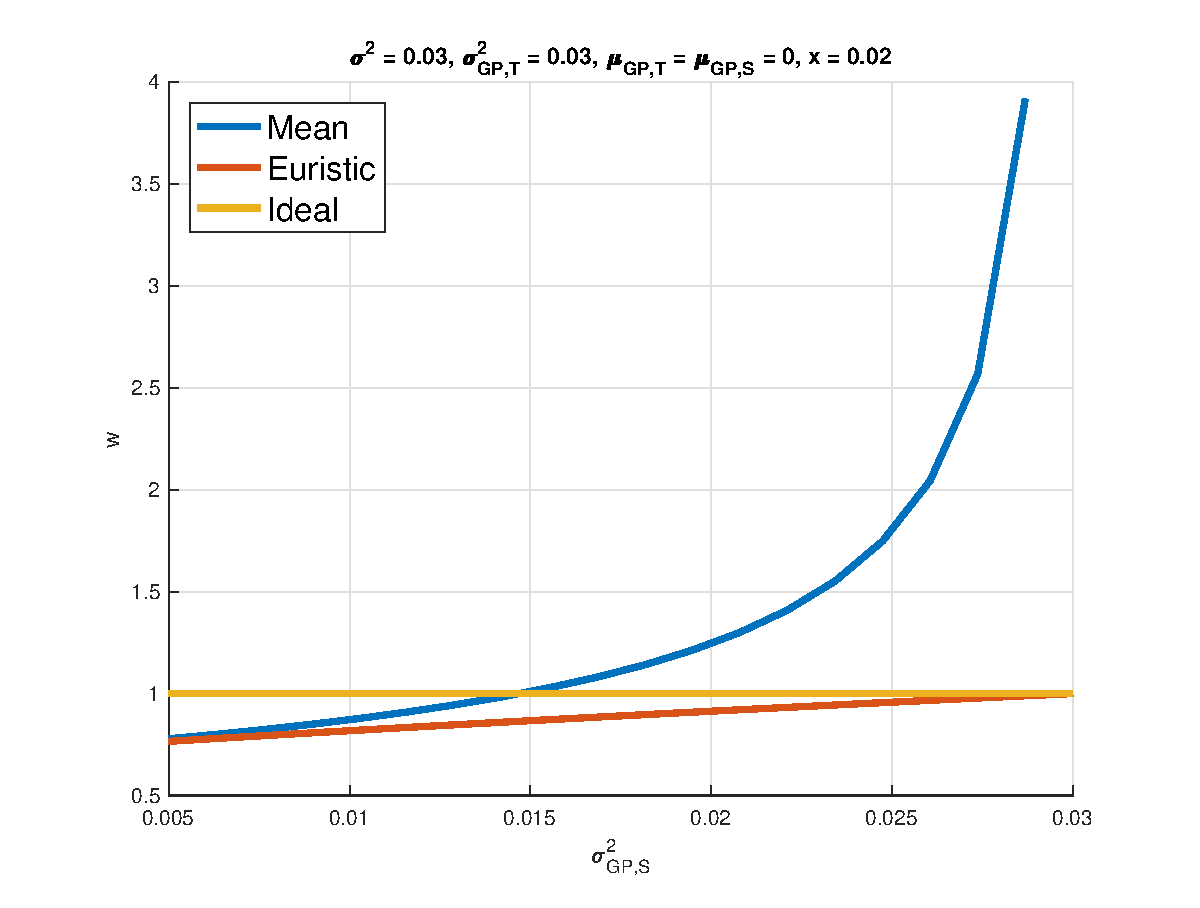
\includegraphics[scale=0.7]{images/weights-plot.eps}
      \caption{Weight estimations according to Equation \ref{mean-weight} (red), \ref{eur} (blue) and the ideal weight (orange)}
      \label{weight-plot}
    \end{figure}

    \noindent A pseudocode implementation of the procedures to estimate weights for rewards and dynamics, in conjunction with
    use \ref{eur}, are given by
    Algorithm \ref{rw_weight_est} and \ref{rw_transition_est}.

    \begin{algorithm}
        \caption{$w_r$ estimation algorithm}\label{rw_weight_est}
        \begin{algorithmic}[1]
          \Procedure{EstimateRwWeight($(s,a,s',r)$, ${GP}_{r}$, $x$)}{}
            \State $W \gets \emptyset$
            \State $\mathcal{N}_{S} = (\mu_{GP,S}, \sigma_{GP,S}^{2}) \gets {GP}^{S}_{r}.predict(s,a)$
            \State $\mathcal{N}_{T} = (\mu_{GP,T}, \sigma_{GP,T}^{2}) \gets {GP}^{T}_{r}.predict(s,a)$
            \For {$i = 0$ $\text{to}$ $N_{samp}$}
              %\State $s_s \gets \mathcal{N}_{s}.sample()$
              %\State $s_t \gets \mathcal{N}_{t}.sample()$
              \State $d_s \gets \mathcal{N}(r; \mu_{GPs}, \sigma^{2}_{r} + \sigma_{GPs}^{2})$
              \State $d_t \gets \mathcal{N}(r; \mu_{GPt}, \sigma^{2}_{r} + \sigma_{GPt}^{2})$
              \State $w_r \gets \frac{d_t}{d_s}$
              \State $W += w_r$
            \EndFor
          \EndProcedure
        \end{algorithmic}
    \end{algorithm}

    \begin{algorithm}
        \caption{$w_p$ estimation algorithm}\label{rw_transition_est}
        \begin{algorithmic}[1]
          \Procedure{EstimateTrWeight($(s,a,s',r)$, ${GP}_{t}$)}{}
            \State $W \gets \emptyset$
            \State $\mathcal{N}_{S} = (\mu_{GP,S}, \sigma_{GP,S}^{2}) \gets {GP}^{S}_{p}.predict(s,a)$
            \State $\mathcal{N}_{T} = (\mu_{GP,T}, \sigma_{GP,T}^{2}) \gets {GP}^{T}_{p}.predict(s,a)$
            \For {$i = 0$ $\text{to}$ $N_{samp}$}
              %\State $s_s \gets \mathcal{N}_{s}.sample()$
              %\State $s_t \gets \mathcal{N}_{t}.sample()$
              \State $d_s \gets \mathcal{N}(s'; \mu_{GPs}, \sigma^{2}_{r} + \sigma_{GPs}^{2})$
              \State $d_t \gets \mathcal{N}(s'; \mu_{GPt}, \sigma^{2}_{r} + \sigma_{GPt}^{2})$
              \State $w_p \gets \frac{d_t}{d_s}$
              \State $W += w_p$
            \EndFor
          \EndProcedure
        \end{algorithmic}
    \end{algorithm}

    \noindent It is also important to notice that the procedure described above is just a possible way to deal with the
    problem of weight estimation. As we will see in the next chapter the learning algorithm (Weighted Fitted Q-Iteration)
    is totally independent of the method used to calculate the weights associated with the sample. This, in our opinion,
    represents a further advantage with respect other transfer learning related algorithms.

  \chapter{Theoretical Analysis}
  \lettrine[lines=2]{I}n this chapter we try to provide some theoretical basis regarding our approach to
  the problem of transfer. In particular we first try to understand if it is possible to provide some
  theoretical bounds to the error introduced by both the use of source samples and the estimation of the
  weights of rewards and dynamics. We are able to show that, under very simple hypothesis, over the tasks
  it possible to bound the bias introduced by the use of source samples in conjunction with estimated weights.

  \section{Errors Bounding}
    \subsection{Assumptions}
      \noindent Suppose $P^{S}(s,a,s',r) = P^{S}(r|s,a)P^{S}(s'|s,a)P^{S}(s,a)$ is the joint density of the samples
      under the source model, and $P^{T}$ the corresponding density under the target model. Let indicate with $x$ either
      the reward $r$ or $s'$ for a given sample $(s,a,s',r)$.
      Suppose, without loss of generality, that only one source MDP exists, indeed, in the case multiple
      source tasks are available no substantial modifications are needed given that no relationship are
      assumed to exists between tasks.
      Any regressor we could adopt in our Weighted Fitted Q-Iteration algorithm tries to minimize the expectation
      of some loss function $L$ under the target distribution:

      \begin{equation}
        arg\min_{\theta} \mathbb{E}_{P^{T}} \left [ L(\hat{Q}_{\theta}^{1} (s,a) + \max_{a'} \hat{Q}_{t-1}(s',a')) \right ]
      \end{equation}
      \noindent This can be computed under the source distribution by employing importance sampling:
      \begin{equation}
        arg\min_{\theta} \mathbb{E}_{P^{S}} \left [ w_{p}(s,a,s') L(\hat{Q}_{\theta}^{1} (s,a) + \max_{a'} \hat{Q}_{t-1}(s',a')) \right ]
      \end{equation}
      where:
      \begin{equation}
        w_{p}(s,a,s') = \frac{P^{T}(s'|s,a) P^{T}(s,a)}{P^{S}(s'|s,a)P^{S}(s,a)}
      \end{equation}
      According to our approach, we neglect the terms $P(s,a)$ and, thus, consider the importance weights defined by:
      \begin{equation}
        w_{p}(s,a,s') = \frac{P^{T}(s'|s,a)}{P^{S}(s'|s,a)}
      \end{equation}
      Notice that this approximation does not introduce any error in the estimation of the Q-function since,
      for every pair $(s,a)$, the target $\hat{Q}^{1} + \max_{a'}\hat{Q}_{t-1}(s',a')$ is always correctly
      weighted.\newline
      \noindent We consider Gaussian models for both the reward and the transitions dynamics, thus:
      \begin{equation}
        P^{T}(r|s,a) = \mathcal{N}(\mu_{r,T}, \sigma_{r}^{2}), \quad P^{S}(r|s,a) = \mathcal{N}(\mu_{r,S}, \sigma^{2}_{r})
      \end{equation}
      and:
      \begin{equation}
        P^{T}(s'|s,a) = \mathcal{N}(\mu_{p,T}, \sigma_{p}^{2}), \quad P^{S}(s'|s,a) = \mathcal{N}(\mu_{p,S}, \sigma^{2}_{p})
      \end{equation}
      We suppose, without loss of generality, the variances are known and do not change between source and target. Let us
      denote the densities we estimate from the available samples as:
      \begin{equation}
        \tilde{P}^{T}(r|s,a) = \mathcal{N}(\tilde{\mu}_{r,T}, \sigma^{2}_{r}), \quad \tilde{P}^{S}(r|s,a) = \mathcal{N}(\tilde{\mu}_{r,S}, \sigma^{2}_{r})
      \end{equation}
      and:
      \begin{equation}
        \tilde{P}^{T}(s'|s,a) = \mathcal{N}(\tilde{\mu}_{p,T}, \sigma^{2}_{p}), \quad \tilde{P}^{S}(s'|s,a) = \mathcal{N}(\tilde{\mu}_{p,S}, \sigma^{2}_{p})
      \end{equation}
      Suppose to have $N$ target samples and $M$ source samples (typically $N << M$). Then, the empirical expected loss considered by
      our regressor is:
      \begin{equation}
        \hat{L} = \frac{1}{N+M}\sum_{i=1}^{N} L(r_i,s'_i) + \frac{1}{N+M} \sum_{j=1}^{M} \tilde{w}_{p}(s'_j)L(r_j, s'_j)
      \end{equation}
      With $\tilde{w}$ we indicated the estimated weights. Notice that we keep the dependency on $(s,a)$ implicit for ease of
      notation.

      \subsection{Analysis}
      \noindent In this section we assume that the state space and the reward function are bounded, anyway the analysis is
      possible also in the unbounded case but less powerful results.

      \begin{equation*}
        \forall s \in \mathcal{S} : s \in [-S,S], \quad \forall (s,a) \in \mathcal{S} \times \mathcal{A} : \mathcal{R}(s,a) \in [-R,R]
      \end{equation*}

      \noindent Under these hypothesis we can prove the following result:

      \begin{lemma} The true importance weights are bounded:
        \begin{equation}
          w(x) \leq W < \infty
        \end{equation}
      \end{lemma}
      \begin{proof}
        The importance weights can be written as:
        \begin{equation}
            w(x) = \frac{P^{T}(x)}{P^{S}(x)}
        \end{equation}
        Let us bound $w(x)$ using the Gaussian hypothesis:
        \begin{equation}
          \begin{aligned}
              & w(x) = exp \left ( \frac{2x(\mu_{x,T} - \mu_{x,S}) - (\mu^{2}_{x,T} - \mu^{2}_{x,S})}{2\sigma^{2}_{x}} \right ) \\
              & = \frac{exp \left ( \frac{2x(\mu_{x,T} - \mu_{x,S})}{2\sigma^{2}_{x}} \right )}{exp \left ( \frac{(\mu^{2}_{x,T} - \mu^{2}_{x,S})}{2\sigma^{2}_{x}} \right )} \\
              & \leq \frac{1}{exp \left ( \frac{(\mu^{2}_{x,T} - \mu^{2}_{x,S})}{2\sigma^{2}_{x}} \right )} \max \left \{ exp \left ( \frac{2X(\mu_{x,T} - \mu_{x,S})}{2\sigma_{x}^{2}} \right ), exp \left ( - \frac{2X(\mu_{x,T} - \mu_{x,S})}{2\sigma_{x}^{2}} \right ) \right \} \\
              & = \frac{exp \left ( \frac{X|\mu_{x,T} - \mu_{x,S}|}{\sigma^{2}_{x}} \right )}{exp \left ( \frac{(\mu^{2}_{x,T} - \mu^{2}_{x,S})}{2\sigma^{2}_{x}} \right )} \\
              & = W \\
              & < \infty
          \end{aligned}
        \end{equation}
        Where $x$ can indicate either the reward $r$ or the next state $s'$ of a given sample.
      \end{proof}

      \noindent Notice that, in practice, any estimated weight larger than $W$ can be safely omitted or clipped
      to zero since it would correspond to a wrong density estimation, thus justifying our assumption.\newline

      \noindent In the following we proceed to give a bound over $|\hat{L} - \mu_{L}|$. We initially
      assume that the reward models of target and source are identical and no generalization error is introduced
      by the regressor over $\hat{Q}^{1}$. In the second part we also add the error introduced by the regression,
      and use of estimated weights, over the reward.\newline
      Again we consider the empirical loss function:
      \begin{equation}
        \hat{L} = \hat{L}_{T} + \hat{L}_{S} = \frac{1}{N+M} \sum_{i=1}^{N} L(r_i, s'_i) + \frac{1}{N+M} \sum_{j=1}^{M} \tilde{w}_{p}(s'_j)L(r_j,s'_j)
      \end{equation}
      where $L \in [0,1]$. The first term refers to the unbiased samples coming the target task, that, by definition
      have unitary weights. The second term refers to the biased samples coming from the source task and must be
      corrected using the corresponding importance weights.\newline

      \noindent Our goal is to find a bound on $|\hat{L} - \mu_{L}|$. This can be easily obtained by simple
      algebraic manipulations of the previous equation:
      \begin{equation}
        \begin{aligned}
          & \left | \hat{L} - \mu_{L} \right | = \left | \hat{L}_{T} - \frac{N}{M+M} \mu_{L} + \hat{L}_{S} - \frac{M}{N+M} \mu_{L} \right | \\
          & \leq \left | \hat{L}_{T} - \frac{N}{N+M} \mu_{L} \right | + \left | \hat{L}_{S} - \frac{M}{N+M} \mu_{L} \right | \\
          & \leq \left | \mathbb{E}_{P^T}[\hat{L}_{T}] - \frac{N}{N+M} \mu_{L} \right | + \left | \hat{L}_{T} - \mathbb{E}_{P^T}[\hat{L}_{T}] \right | \\
          & + \left | \mathbb{E}_{P^S} [\hat{L}_{S}] - \frac{M}{N+M} \mu_{L} \right | + \left | \hat{L}_{S} - \mathbb{E}_{P^S} [\hat{L}_{S}] \right | \\
          & = \left | \hat{L}_{T} - \mathbb{E}{P^T}[\hat{L}_{T}] \right | + \left | \mathbb{E}_{P^S}[\hat{L}_{S}] - \frac{M}{M+N}\mu_{L} \right | + \left | \hat{L}_{S} - \mathbb{E}_{P^{S}} [\hat{L}_{S}] \right |
        \end{aligned}
      \end{equation}
      where the last equality holds since the first term is zero (the estimator $\hat{L}_{T})$ is unbiased). We now proceed to
      bound the three terms separately:

      \begin{lemma}
        Given $\delta > 0$, with probability at least $1 - \delta$, the term $\left | \hat{L}_{T} - \mathbb{E}_{P^T} [\hat{L}_{T}] \right |$ is
        bounded by:
        \begin{equation}
          \left | \hat{L}_{T} - \mathbb{E}_{P^T} [\hat{L}_{T}] \right | \leq \frac{2\log(2/\delta)}{3(N+M)} + \sqrt{\frac{N\log(2/\delta)}{2(N+M)^{2}}}
        \end{equation}
        \label{lemma5}
      \end{lemma}
      \begin{proof}
        From Bernstein's inequality, we know that:
        \begin{equation}
          P \left ( \left | \sum_{i=1}^{N} L_{i} - N\mathbb{E}_{P^{T}}[L] \right | > t \right ) < 2 exp \left ( -\frac{t^{2}/2}{N Var[L] + Ct/3} \right )
        \end{equation}
        By setting $t = (N+M)\epsilon$, we obtain:
        \begin{equation}
          P \left ( \left | \hat{L} - \mathbb{E}[\hat{L}] \right | > \epsilon \right ) < 2 exp \left ( -\frac{(N+M)^{2}\epsilon^{2}/2}{N Var[L] + (N+M)C \epsilon /3} \right )
        \end{equation}
        Notice that $C$, ie. the range of $L$, is 1, and, from Popoviciu's inequality, $Var[L] \leq 1/4$. By setting
        the right-hand side equal to $\delta$ and solving for $\epsilon$, we obtain the desired result.
      \end{proof}

      \begin{lemma}
        Given $\delta > 0$, with probability at least $1-\delta$, the term $\left | \hat{L}_{S} - \mathbb{E}_{P^S}[\hat{L}_{S}] \right |$
        is bounded by:
        \begin{equation}
          \left | \hat{L}_{S} - \mathbb{E}_{P^S}[\hat{L}_{S}] \right | \leq \frac{2W\log(2/\delta)}{3(N+M)} + \sqrt{\frac{2MW^{2}\log(2/\delta)}{(N+M)^{2}}}
        \end{equation}
        \label{lemma6}
      \end{lemma}
      \begin{proof}
        The proof follows straightforwardly from the one of Lemma \ref{lemma5}. Simply notice that now the range of $\tilde{w}_{p}(s')L(r,s')$
        is $C = W$ and a trivial bound on its variance is $Var[\tilde{w}_{p}(s')L(r,s')] \leq W^{2}$.
      \end{proof}

      \begin{lemma}
        The term $\left | \mathbb{E}_{P^S} [\hat{L}_{S}] - \frac{M}{N+M}\mu_{L} \right |$ is bounded by:
        \begin{equation}
          \left | \mathbb{E}_{P^S} [\hat{L}_{S}] - \frac{M}{N+M}\mu_{L} \right | \leq \frac{M}{N+M}
        \end{equation}
        \label{lemma7}
      \end{lemma}
      \begin{proof}
        Notice that we can write:
        \begin{equation}
          \begin{aligned}
            & \left | \mathbb{E}[\hat{L}_{S}] - \frac{M}{N+M}\mu_{L} \right | = \left | \frac{M}{N+M} \mathbb{E}[\tilde{w}_{p}(s')L(s')] - \frac{M}{M+N}\mu_{L} \right | \\
            & \qquad = \frac{M}{N+M} | \mathbb{E}_{P^S}[\tilde{w}_{p}(s')L(s') - w_{p}(s')L(s')]|
          \end{aligned}
          \label{bound1}
        \end{equation}

        The latter term can be bound with:
        \begin{equation}
          \begin{aligned}
            & |\mathbb{E}_{P^S}[\tilde{w}_{p}(s')L(s') - w_{p}(s')L(s')]| \\
            & \qquad =    \left | \mathbb{E}_{P^{S}} \left [ \frac{\tilde{P}^{T}(s')}{\tilde{P}^{S}(s')}L(s') \right ] - \mathbb{E}_{P^{S}} \left [ \frac{P^{T}(s')}{P^{S}(s')}L(s') \right ] \right | \\
            & \qquad \leq \left | \mathbb{E}_{P^{S}} \left [ \frac{\tilde{P}^{T}(s')}{\tilde{P}^{S}(s')}L(s') \right ] - \mathbb{E}_{P^{S}} \left [ \frac{\tilde{P}^{T}(s')}{P^{S}(s')}L(s') \right ] \right | \\
            & \qquad + \left | \mathbb{E}_{P^{S}} \left [ \frac{\tilde{P}^{T}(s')}{P^{S}(s')}L(s') \right ] - \mathbb{E}_{P^{S}} \left [ \frac{P^{T}(s')}{P^{S}(s')}L(s') \right ] \right | \\
            & \qquad = \left | \mathbb{E}_{P^{S}} \left [ \frac{\tilde{P}^{T}(s')}{\tilde{P}^{S}(s')P^{S}(s')} \left ( P^{S}(s')L(s') - \tilde{P}^{S}(s')L(s') \right ) \right ] \right | \\
            & \qquad + \left | \mathbb{E}_{P^S} \left [ \frac{1}{P^{S}(s')} \left ( \tilde{P}^{T}(s')L(s') - P^{T}(s')L(s') \right ) \right ] \right | \\
            & \qquad = \left | \int \tilde{w}_{p}(s') \left ( P^{S} (s') L(s') - \tilde{P}^{S}(s')L(s')\right ) ds' \right | \\
            & \qquad + \left | \int \left ( P^{T}(s')L(s') - \tilde{P}^{T}(s')L(s') \right ) ds' \right | \\
            & \qquad \leq 2W\mathcal{TV}(P^{S}||\tilde{P}^{S}) + 2\mathcal{TV}(P^{T}||\tilde{P}^{T})
          \end{aligned}
        \end{equation}
        where $\mathcal{TV}$ denotes the \textit{total variation distance} between two probability measures. Remember that the
        total variation can be written as:
        \begin{equation}
          \mathcal{TV}(p||q) = \frac{1}{2} \sup_{f:|f|<1} \left | \int (f(x)p(x) - f(x)q(x)) dx \right |
        \end{equation}

        \noindent This last equation can be further expanded by considering Pinsker's inequality:
        \begin{equation}
          \begin{aligned}
            & 2W\mathcal{TV}(P^{S}||\tilde{P}^{S}) + 2\mathcal{TV}(P^{T}||\tilde{P}^{T}) \\
            & \leq 2W \sqrt{\frac{1}{2} \mathcal{KL}(P^{S}||\tilde{P}^{S})} + 2\sqrt{\frac{1}{2}\mathcal{KL}(P^{T}||\tilde{P}^{T})} \\
            & \leq 2W \sqrt{\frac{|\mu_{p,S} - \tilde{\mu}_{p,S}|^{2}}{4\sigma^{2}_{p}}} + 2\sqrt{\frac{|\mu_{p,T} - \tilde{\mu}_{p,T}|^{2}}{4\sigma^{2}_{p}}} \\
            & \leq W \frac{|\mu_{p,S} - \tilde{\mu}_{p,S}|}{\sigma_{p}} + \frac{|\mu_{p,S} - \tilde{\mu}_{p,S}|}{\sigma_{p}}
          \end{aligned}
        \end{equation}
        where $\mathcal{KL}$ is the Kullback-Leibler divergence. By combining the latter bound with Equation \ref{bound1} we obtain the
        desired result.
      \end{proof}

      \noindent Finally, by combining the previous result we obtain the final result:
      \begin{theorem}
        Given $\delta > 0$, with probability at least $1-2\delta$:
        \begin{equation}
          \begin{aligned}
            & \left | \hat{L}-\mu_{L} \right | \leq \frac{2\log(2/\delta)}{3(N+M)} + \sqrt{\frac{N\log(2/\delta)}{2(N+M)^{2}}} + \frac{2W\log(2/\delta)}{3(N+M)}+ \sqrt{\frac{2MW^{2}\log(2/\delta)}{(N+M)^{2}}} \\
            & \qquad \quad + \frac{M}{N+M} \left ( W \frac{|\mu_{p,S} - \tilde{\mu}_{p,S}|}{\sigma_{p}} + \frac{|\mu_{p,S} - \tilde{\mu}_{p,S}|}{\sigma_{p}} \right )
          \end{aligned}
        \end{equation}
      \end{theorem}
      \begin{proof}
        The proof is an immediate conseguence of Lemma \ref{lemma5}, \ref{lemma6} and \ref{lemma7}.
      \end{proof}
      \vspace{2cm}

      \noindent The last bound is very loose but provides some useful insights. When the predictions of the GPs are
      perfect and $M, N \rightarrow \infty$ then $|\hat{L}-\mu_{L}| \rightarrow 0$. In practice we have that when,
      the number of source samples is sufficiently high, the predictions of the GPs precise and a good generalization
      from the regressor used in WFQI, the bias introduced by the use of biased samples with estimated importance
      weights is reasonably low.\newline

      \noindent We could also consider the bias introduced by the use of $\hat{Q}^{1}(s,a)$ in place of the reward coming from the
      experience sample. This error is composed of two parts: the first one is due to the generalization error introduced
      by the specific regressor used in WFQI, the second part, again, is given by the use of estimated weights for the
      reward model and can be studied with an analysis analogous to the one of the transition model. Notice this
      bound does not provide any insight on how the errors propagate in different iterations of WFQI.\newline

      \noindent The next chapter is devoted to the empirical validation of the theoretical results presented
      so far. We observe how different number of source and target sample affects the performance of WFQI and
      appears to be always respectful of the results obtained in this chapter.

  \chapter{Experimental Results}
  \noindent This chapter is devoted to the experimental evaluation of WFQI on classic RL problems.
  We test the proposed algorithm on two versions of the puddle world and on the activity swing-up. Both
  environments have a continuous state-space and discrete action-space. We evaluate the performance of WFQI in terms
  of expected return under different numbers of source/target samples varying also the number of source tasks involved.\newline
  We start presenting the metrics we adopt to evaluate our approach and finally, we report the results over
  the different environments.

  \section{Evaluation Metrics}
    \noindent Defining a metric for the notion the notion of "good transfer" is, in general, a hard task and
    in literature different metrics have been proposed. As already highlighted in the previous section
    we plot the results in terms of expected discounted return $J_{\pi}$ of the best policy learnt by WFQI
    after performing the transfer:
    \begin{equation}
      J_{\pi} = \sum_{t=0}^{T} \gamma^{t}R(s_{t}, \pi(s_{t}))
    \end{equation}
    The resulting graphs are quite useful because they permit to have a graphical overview
    of the jumpstart improvement and of the time to learn the optimal policy from the source
    and target samples.\newline

  \section{The Puddle World Environment}
    \noindent In this set of experiments we deal with MDPs with continuous state space (and discrete action space).\newline
    Puddle-world is an environment similar to grid-world where the agent must move toward a safe area while avoiding
    to walk inside the puddles. Only four actions (N,S,W,E) are allowed in each state. When the agent bump in the
    border of the environment it always return to the state where the action was initially performed.\newline
    The settings for the experiment is the following: two task (target and source), $\gamma = 0.99$, the size is $10 \times 10$,
    and the maximum horizon is set to 30 iterations.\newline

    \noindent Puddles are modeled as (inverse) bivariate gaussian:
    \begin{equation}
      \begin{multlined}
        P(x,y) = - \frac{1}{2 \pi \sigma_x \sigma_y \sqrt{1 - \rho}} e^{-\frac{z}{2(1-\rho)^{2}}} \\
        z = \frac{(x - \mu_x )^2}{\sigma_x^2} - \frac{2 \rho (x-\mu_x)(y-\mu_y)}{\sigma_x \sigma_y} + \frac{(y - \mu_y )^2}{\sigma_y^2} \\
        \rho = \frac{\sigma_{xy}}{\sigma_x \sigma_y} \\
      \end{multlined}
    \end{equation}

    \begin{figure}[H]
      \centering
      \includegraphics[scale=0.6]{images/puddleex.eps}
      \caption{An example puddle world environment, in red the FQI policy.}
      \label{puddleex}
    \end{figure}

    \noindent We propose two variations of the puddle world environment: in the first one when the agent comes close to a puddle he
    receives a penalty proportional to the distance from the centre of the puddle; in the second variation when the agent come close
    to a puddle the length of the step reduces proportionally with respect to the distance from the center of the puddle.\newline

    \noindent In the first variation the reward for $(s,a)$ is given by the following set of equations. Let be $\mathcal{U}$ the set of puddles then:
    \begin{equation}
      r(s,a) =
      \begin{cases}
        \mathcal{N}(0,0.01) + \sum_{u \in \mathcal{U}} 100 P_{u}(s') & s' \textit{ is at goal} \\
        -1 + \mathcal{N}(0,0.01) + \sum_{u \in \mathcal{U}} 100 P_{u}(s') & s' \textit{ otherwise} \\
      \end{cases}
      \label{rw-puddle}
    \end{equation}
    The dynamics is simply given by modifying deterministically the coordinates of $s$ depending on the action $a$ chosen by
    the agent, the step-lenght $\alpha$ is unitary. Finally we add a Gaussian noise $\mathcal{N}(0,0.04)$ to both the coordinates
    to obtain $s'$.\newline

    \noindent In the second variation the reward is still given by Equation \ref{rw-puddle}, but the dynamics is now dependent also
    on the position of the agent. In particular $\alpha$ is no more unitary but given by the following equation:
    \begin{equation}
      \alpha = \frac{1}{1 + 30\sum_{u \in \mathcal{U}} P_{u}(s')}
    \end{equation}
    When the agent comes closer to the center of a puddle $\alpha \rightarrow 0$.

  \section{Target and Sources Tasks}
    \noindent In this section, we present the tasks involved in the experiments. The source tasks have different degrees
    of similarity with respect to the target task. The source task 3 (figure \ref{source3}) has the highest similarity
    but the puddles are slightly misplaced and the goal region is smaller and shifted on the right of the space. The source
    task 1 (figure \ref{source1}) maintains some similarities with the target but a large puddle on the bottom-left corner
    may produce very different policies. The last source task (figure \ref{source2}) is the one that has the highest
    differences with respect to the target, indeed the puddle configuration is very different.

    \begin{figure}[H]
      \centering
      \includegraphics[scale=0.6]{images/target.pdf}
      \caption{The target task used in the experiments, in red the FQI policy.}
      \label{target}
    \end{figure}
    %
    \begin{figure}[H]
      \centering
      \includegraphics[scale=0.6]{images/source1.eps}
      \caption{Source task 1 used in the experiments, in red the FQI policy.}
      \label{source1}
    \end{figure}
    %
    \begin{figure}[H]
      \centering
      \includegraphics[scale=0.6]{images/source2.eps}
      \caption{Source task 2 used in the experiments, in red the FQI policy.}
      \label{source2}
    \end{figure}
    %
    \begin{figure}[H]
      \centering
      \includegraphics[scale=0.6]{images/source3.eps}
      \caption{Source task 3 used in the experiments, in red the FQI policy.}
      \label{source3}
    \end{figure}
    %

  \section{Results - Puddle World Version 1}
    \noindent This version of puddle world is meant to test the reward transfer capability of the algorithm. In this scenario when the
    agent comes closer to a puddle it receives a penalty on the reward proportional to the distance with respect
    to the centre of the puddle. The dynamics of the agent are unchanged (ie. the step remains unitary).\newline
    From the perspective of the weight calculation this means that only the weight associated with the reward needs to be estimated,
    the weights associated with the dynamics are always unitary.\newline
    In the following experiments, the results are averaged over 50 runs, the initial position of the agent is randomized
    at each run in the area $[0,2][0,2]$.\newline

    \noindent The parameters for the tree-based WFQI algorithm are: 50 estimators, 5 random splits and 2 minimum samples per leaf.
    Source samples are collected using the red policies reported in the previous figures.

    \subsection{Ideal Weights}
    \noindent For this set of experiments we assume to be able to calculate the ideal weights, that is we assume
    to perfectly know the model of the reward (the dynamics are identical in both the source and target task).
    Given a perfect knowledge of the model of the environment, it is possible to obtain a perfect estimation of
    the weights leading to an unbiased use of the source samples in the target task.

    \begin{figure}[H]
      \centering
      \includegraphics[scale=0.5]{images/WFQIPerf1_ID.eps}
      \caption{WFQI performance Source 1/Target task, ideal weights}
      \label{perf1ID}
    \end{figure}
    %
    \begin{figure}[H]
      \centering
      \includegraphics[scale=0.5]{images/WFQIPerf2_ID.eps}
      \caption{WFQI performance Source 2/Target task, ideal weights}
      \label{perf2ID}
    \end{figure}
    %
    \begin{figure}[H]
      \centering
      \includegraphics[scale=0.5]{images/WFQIPerf3_ID.eps}
      \caption{WFQI performance Source 3/Target task, ideal weights}
      \label{perf3ID}
    \end{figure}
    %

    \noindent In this last set of experiments the samples are transferred from all
    the source tasks toward the target in equal quantities.

    \begin{figure}[H]
      \centering
      \includegraphics[scale=0.5]{images/WFQIPerfM_ID.eps}
      \caption{WFQI performance Source 1/2/3/Target task, ideal weights}
      \label{perfMID}
    \end{figure}
    %

    \noindent The results reflect the theoretical expectation: the best performances are achieved
    with the source tasks 1 and 3, on the other side, the source task 2 appear to be of little help.\newline
    Another important observation is that our algorithm is successfully able
    to limit the phenomena of the negative transfer; indeed the performance in figure \ref{perfMID}
    seems to not be influenced by the bad sample present in the source task 2.

    \subsection{Estimated Weights}
    \noindent For this set of experiments we assume to be not able to calculate the ideal weights, they are calculated
    using algorithm \ref{rw_weight_est}. These algorithms provide only an
    estimation of the real weights, therefore the use of the corresponding source samples in the target
    task is not perfectly unbiased (as in the previous scenario). A theoretical bounds over the introduced
    error has been given in the next chapter. Weights are estimated according to Equation \ref{eur}.

    \begin{figure}[H]
      \centering
      \includegraphics[scale=0.5]{images/WFQIPerf1.eps}
      \caption{WFQI performance Source 1/Target task, est. weights}
      \label{perf1E}
    \end{figure}
    %
    \begin{figure}[H]
      \centering
      \includegraphics[scale=0.5]{images/WFQIPerf2.eps}
      \caption{WFQI performance Source 2/Target task, est. weights}
      \label{perf2E}
    \end{figure}
    %
    \begin{figure}[H]
      \centering
      \includegraphics[scale=0.5]{images/WFQIPerf3.eps}
      \caption{WFQI performance Source 3/Target task, est. weights}
      \label{perf3E}
    \end{figure}
    %

    \noindent In this last set of experiments the samples are transferred from all
    the source tasks toward the target in equal quantities.

    \begin{figure}[H]
      \centering
      \includegraphics[scale=0.5]{images/WFQIPerfM.eps}
      \caption{WFQI performance Source 1/2/3/Target task, est. weights}
      \label{perfME}
    \end{figure}

    \vspace{3cm}
    %

    \noindent Again he results reflects the theoretical expectation: the best performances are achieved
    with the source tasks 1 and 3, on the other side the source task 2 appear to be of little help.\newline
    Also in this situation our algorithm is able to maintain the ability to successfully
    limit the phenomena of the negative transfer; indeed the performance in figure \ref{perfME}
    seems to not be influenced by the bad sample present in Source task 2.\newline

    \noindent In addition we provide the results obtained using Equation \ref{mean-weight} using
    the correct and an overestimated value for $\sigma^{2}$. The task at hand is very simple but
    we can notice, in the case we do not fake the value of $\sigma^{2}$, a poor performance
    when the number of source samples is low. This effect is due to the fact that when $\sigma_{GP,S}^{2}$
    is high formula \ref{mean-weight} produces a very imprecise estimation of the weights.

    \begin{figure}[H]
      \centering
      \includegraphics[scale=0.6]{images/WFQIPerfM_V1_MEAN.eps}
      \caption{Performance over Puddle-World V1, no $\sigma^{2}$ overestimation, $\sigma^{2} = 0.01$, multiple source tasks}
      \label{}
    \end{figure}

    \begin{figure}[H]
      \centering
      \includegraphics[scale=0.5]{images/WFQIPerfM_V1_MEAN2.eps}
      \caption{Performance over Puddle-World V1, with $\sigma^{2}$ overestimation, $\sigma^{2} = 0.09$, multiple source tasks}
      \label{}
    \end{figure}


    \noindent As a final remark notice that using a weight $w = w_r*w_p$ in this environment would be
    of great disadvantage. Indeed here we assume that the transition model does not change between
    source and target task while the reward model can change arbitrary. This means we can assume
    $w_p = 1$ while the value of $w_r$ can change depending on the specific sample. If the source task
    is significantly different from the target it means that $w$ will assume a low value in the entire
    state-action space thus limiting the transfer. On the other hand with our approach, where reward weights
    are only used in the first iteration and transition weights are used in the remaining, the transfer
    procedure can fully exploit the similarities of the dynamics and thus maximizes the number of transferred
    samples.


  \section{Results - Puddle World Version 2}
    \noindent This environment is a variation of the previous puddle world, in this scenario when the agent is
    close to a puddle in addition to the reward penalty it also modifies its step length that decreases
    proportionally to the distance with respect to the center of the puddle. This situation is much more
    complicated from the transfer perspective: in addition to the weight necessary for the reward model, in
    this case we need to compute a weight also for the transfer of the dynamics of the agent (that now are
    changed).

    \subsection{Ideal Weights}
    \noindent In the first set of experiments we test the performance of WFQI using the ideal weights,
    that is we assume to perfectly know the stochastic model for both the reward and transition model.
    As expected we obtain over the single task transfer an almost perfect performance, meaning that also
    with a very small amount of transferred source samples we reach the score achieved by the optimal policy.\newline

    \noindent The parameters for the tree-based WFQI algorithm are: 50 estimators, 2 random splits and 1 minimum samples per leaf.

    \begin{figure}[H]
      \raggedbottom
      \centering
      \includegraphics[scale=0.5]{images/WFQIPerf1_ID_V2.eps}
      \caption{WFQI performance Source 1/Target task, ideal weights}
      \label{perf1E}
    \end{figure}
    %
    \begin{figure}[H]
      \raggedbottom
      \centering
      \includegraphics[scale=0.5]{images/WFQIPerf2_ID_V2.eps}
      \caption{WFQI performance Source 2/Target task, ideal weights}
      \label{perf2E}
    \end{figure}
    %
    \begin{figure}[H]
      \raggedbottom
      \centering
      \includegraphics[scale=0.5]{images/WFQIPerf3_ID_V2.eps}
      \caption{WFQI performance Source 3/Target task, ideal weights}
      \label{perf3E}
    \end{figure}
    %

    \noindent In this last set of experiments the samples are transferred from all
    the source tasks toward the target in equal quantities. Again we highlight the
    fact that despite the fact that samples coming from the second source task
    are not effective for the transfer, the algorithm is able to completely
    eliminate the negative transfer and to reach the maximum performance.

    \begin{figure}[H]
      \raggedbottom
      \centering
      \includegraphics[scale=0.5]{images/WFQIPerfM_ID_V2.eps}
      \caption{WFQI performance Source 1/2/3/Target task, ideal weights}
      \label{perfMIDV2}
    \end{figure}
    %

    \subsection{Estimated Weights}

    \noindent For this set of experiments weights are calculated
    using algorithms \ref{rw_weight_est} and \ref{rw_transition_est}. These algorithms provide only an
    estimation of the real weights, therefore the use of the corresponding source samples in the target
    task is not perfectly unbiased (as in the previous scenario). The performance is not as good as
    in the ideal case due to the error introduced thanks to the estimation of the weights.
    Weights are estimated according to Equation \ref{eur}.

    \begin{figure}[H]
      \raggedbottom
      \centering
      \includegraphics[scale=0.5]{images/WFQIPerf1_V2.eps}
      \caption{WFQI performance Source 1/Target task, est. weights}
      \label{perf1V2}
    \end{figure}
    %

    \begin{figure}[H]
      \raggedbottom
      \centering
      \includegraphics[scale=0.5]{images/WFQIPerf2_V2.eps}
      \caption{WFQI performance Source 2/Target task, est. weights}
      \label{perf2V2}
    \end{figure}
    %

    \begin{figure}[H]
      \raggedbottom
      \centering
      \includegraphics[scale=0.5]{images/WFQIPerf3_V2.eps}
      \caption{WFQI performance Source 3/Target task, est. weights}
      \label{perf3V2}
    \end{figure}
    %

    \noindent In this last set of experiments the samples are transferred from all
    the source tasks toward the target in equal quantities. Also in this case,
    despite the fact that samples coming from the second source task
    are not effective for the transfer, the algorithm is able to eliminate the negative
    transfer effect and to achieve an satisfactory performance.

    \begin{figure}[H]
      \raggedbottom
      \centering
      \includegraphics[scale=0.5]{images/WFQIPerfM_V2.eps}
      \caption{WFQI performance Source 1/2/3/Target task, est. weights}
      \label{perfMV2}
    \end{figure}

    \noindent In addition we also report the results when weights are estimated according to
    Formula \ref{mean-weight} using respectively, in Figure \ref{mean-res1} $\sigma^{2}_r = 0.01$ and
    $\sigma^{2}_{p} = 0.04$ and in Figure \ref{mean-res2} $\sigma^{2}_{r} = 0.09$ and $\sigma^{2}_{p} = 0.36$.

    \begin{figure}[H]
      \centering
      \includegraphics[scale=0.5]{images/WFQIPerfM_V2_MEAN.eps}
      \caption{Puddle-World performance, multiple source tasks, Equation \ref{mean-weight} \textbf{without} $\sigma^{2}$ overestimation}
      \label{mean-res1}
    \end{figure}

    \begin{figure}[H]
      \centering
      \includegraphics[scale=0.5]{images/WFQIPerfM_V2_MEAN2.eps}
      \caption{Puddle-World performance, multiple source tasks, Equation \ref{mean-weight} \textbf{with} $\sigma^{2}$ overestimation}
      \label{mean-res2}
    \end{figure}


    \noindent We observe, in the first case, poor performances, mainly due high number of discarded samples.
    In the second graph we notice a much better performance due to the overestimation of $\sigma^{2}$ for
    both reward and transition model, in this case even better than the heuristic approach.
    %

  \section{Acrobot Environment}
    \noindent Acrobot is a two-link underactuated robot, we refer to the model described by \cite{ernst2005tree}. A
    graphical representation is depicted in figure \ref{acrobot_fig}.

    \begin{figure}[H]
      \raggedbottom
      \centering
      \includegraphics[scale=0.3]{images/acrobot.png}
      \caption{A graphical representation of the Acrobot environment}
      \label{acrobot_fig}
    \end{figure}
    %

    \noindent The state space of the problem is continuous and described by the
    tuple $[\theta_1, \theta_2, \dot{\theta}_1, \dot{\theta}_2]$, where $\theta_1$ and
    $\theta_2$ are the angles of the two links and $\dot{\theta}_1$ and $\dot{\theta}_2$
    are the two corresponding angular speeds. The action space is discrete and the only
    two possibility are to apply a torque of either $-5$ or $5$.\newline
    The goal is to bring as fast as possible the two links in the upright position.
    The reward signal is $-1$ for every action and $0$ when the two links are in the
    neighbourhood of the goal position.\newline

    \noindent The dynamical system equations of the Acrobot are given by:
    \begin{equation}
      \begin{cases}
        d_{11}\ddot{\theta}_1 + d_{12}\ddot{\theta}_2 + c_1 + \phi_1 = -\mu_{1} \dot{\theta}_1 \\
        d_{12}\ddot{\theta}_1 + d_{22}\ddot{\theta}_2 + c_2 + \phi_2 = u - \mu_{2} \dot{\theta}_2 \\
        d_{11} = M_{1}L_{1}^{2} + M_{2}(L_{1}^{2} + L_{2}^{2}  + 2L_{1}L_{2}\cos(\theta_2)) \\
        d_{22} = M_{2}L_{2}^{2} \\
        d_{12} = M_{2}(L_{2}^{2} + 2L_{1}L_{2}\cos{\theta_2}) \\
        c_{1} = -M_{2}L_{1}L_{2}\dot{\theta}_{2}(2\dot{\theta}_{1} + \dot{\theta}_{2})\sin({\theta_2)} \\
        c_{2} = M_{2}L_{1}L_{2}\dot{\theta}_{1}^{2}\sin(\theta_{2}) \\
        \phi_{1} = -(M_{1}L_{1} + M_{2}L_{1}) g \sin(\theta_1) - M_{2}L_{2} g \sin(\theta_1 + \theta_2) \\
        \phi_{2} = -M_{2}L_{2} g \sin(\theta_1 + \theta_2) \\
      \end{cases}
    \end{equation}

    \noindent $g = 9.81 m/s^{2}$ is the gravitational acceleration coefficient while $\mu_1$ and $\mu_2$ are the
    friction coefficients for the corresponding two joints.\newline
    The discount factor $\gamma$ of the corresponding MDP is $0.95$.

    \subsection{Tasks}
      \noindent For the Target task we set $L_1 = 1.0, L_2 = 1.0, M_1 = 1.0, M_2 = 1.0, \mu_1 = 0.1, \mu_2 = 0.1$.\newline
      For the Source task 1 we set $L_1 = 0.9, L_2 = 0.95, M_1 = 0.95, M_2 = 1.0, \mu_1 = 0.1, \mu_2 = 0.1$\newline
      For the Source task 2 we set $L_1 = 0.8, L_2 = 0.6, M_1 = 0.9, M_2 = 1.0, \mu_1 = 0.1, \mu_2 = 0.1$\newline
      For the Source task 3 we set $L_1 = 0.85, L_2 = 0.85, M_1 = 0.9, M_2 = 0.9, \mu_1 = 0.1, \mu_2 = 0.1$\newline

      \noindent Tests are performed singularly, $Source \rightarrow Target$ and in ensemble, $Source 1/2/3 \rightarrow Target$.

    \vspace{10cm}
    \subsection{Results - Acrobot}
    \noindent In this section we report the results relative to the Acrobot environment, tests are performed with the following
    parameters: $Estimators = 50, Random Split = 5, Min. Samples per leaf = 2$, WFQI is executed over 50 iterations,
    the horizon of the MDP is set to 100. Results are averaged of 30 runs.\newline
    It is important to observe the these settings represents a much more difficult than the previous
    experiments: we are no more in a gaussian settings (while in Puddle World the dynamics and rewards models are
    assumed to be normally distributed), this means that the use of GPs introduces a further error (in addition
    to the bias of the estimated weights); despite this further difficulty again we are able to obtain interesting
    advantages from our approach. Weights are estimate according to Equation \ref{eur}.

    \begin{figure}[H]
      \raggedbottom
      \centering
      \includegraphics[scale=0.5]{images/WFQIPerf1_acro.eps}
      \caption{WFQI performance Source 1/Target task, est. weights}
      \label{acro1}
      %
    \end{figure}
    \begin{figure}[H]
      \raggedbottom
      \centering
      \includegraphics[scale=0.5]{images/WFQIPerf2_acro.eps}
      \caption{WFQI performance Source 2/Target task, est. weights}
      \label{acro2}
      %
    \end{figure}
    \begin{figure}[H]
      \raggedbottom
      \centering
      \includegraphics[scale=0.5]{images/WFQIPerf3_acro.eps}
      \caption{WFQI performance Source 3/Target task, est. weights}
      \label{acro3}
    \end{figure}
    %

    \noindent Note that in Source task 2 the performance are lower given that it is very different from the
    target task.\newline
    In the last set of experiments we transfer from all the three source tasks to the target. Again our algorithm
    reveals to be robust toward the effect of the negative transfer (ie. samples from source task 2) and maintains
    an optimal performance using the information coming from the other two.

    \begin{figure}[H]
      \raggedbottom
      \centering
      \includegraphics[scale=0.5]{images/WFQIPerfM_acro.eps}
      \caption{WFQI performance Source 1/2/3/Target task, est. weights}
      \label{acro3}
    \end{figure}

    \noindent In addition we also report the results when weights are estimated according to
    Formula \ref{mean-weight} using respectively, in Figure \ref{acro-mean-res1}
    $\sigma^{2}_{p} = 0.09$ and in Figure \ref{acro-mean-res2} $\sigma^{2}_{p} = 0.81$.

    \begin{figure}[H]
      \centering
      \includegraphics[scale=0.5]{images/WFQIPerfM_acro_MEAN.eps}
      \caption{Acrobot performance, multiple source tasks, Equation \ref{mean-weight} \textbf{without} $\sigma^{2}$ overestimation}
      \label{acro-mean-res1}
    \end{figure}

    \begin{figure}[H]
      \centering
      \includegraphics[scale=0.5]{images/WFQIPerfM_acro_MEAN2.eps}
      \caption{Acrobot performance, multiple source tasks, Equation \ref{mean-weight} \textbf{with} $\sigma^{2}$ overestimation}
      \label{acro-mean-res2}
    \end{figure}

    \noindent We observe, in the first case, poor performances, mainly due high number of discarded samples.
    In the second graph we notice a much better performance due to the overestimation of $\sigma^{2}$ for
    both reward and transition model. However notice, in this case, that the performance is not as good as
    in Figure \ref{acro3}. This is mainly due to the fact that Acrobot is a non-gaussian environment
    and $\sigma^{2}$ is just the result of an educated guess and may be not the best choice for this specific
    scenario. Better results could be obtained by using some estimation procedures for $\sigma^{2}$.

  \section{Comparison}
    \noindent In this section we compare our approach with the one presented in \cite{lazaric2008transfer} (abbreviated as BATCH). This
    last approach is based on the calculation of measures between tasks and samples. When the target and source
    tasks share some similarities (in this case the authors assume the tasks to be drawn from the same probability
    distribution $\Omega$) it is possible to measure the distance (called task compliance) between a target and
    a source task, moreover within each source we can measure the likelihood of each sample (sample relevance) to be generated
    in the target task. The algorithm first calculate for each source task the compliance and then for each sample of
    each source, it calculates the relevance. Samples are drawn from each task proportionally to the calculated compliance
    and relevance. For more detail we remand to \cite{lazaric2008transfer}.\newline

    \noindent We compare the performance of WFQI and BATCH over the two environments defined before (Puddle-World and Acrobot).\newline
    For Puddle-World, we use a total of 1000 source samples extracted from the three source tasks at hand. For WFQI the parameters
    are identical to the ones presented in the previous section. For BATCH we maintain the same parameters reported in \cite{lazaric2008transfer}.
    For WFQI calculate weights using the overestimation of $\sigma^{2}$ (in particular we take $\sigma^{2} = 0.09$).

    \begin{figure}[H]
      \centering
      \includegraphics[scale=0.5]{images/WFQIPerfCMP.eps}
      \caption{Puddle World - Performance comparison BATCH vs WFQI}
      \label{}
    \end{figure}


    \noindent Notice how our approach is able to gain a better jumpstart performance over BATCH when the number of target samples is low.\newline

    \noindent Moreover we propose a similar comparison also over the Acrobot environment. In this case 1000 source samples are used,
    parameters for WFQI are unchanged with respect to the previous case. For BATCH we use ($\delta_{s,a}=0.3, \delta_{r}=0.5, \delta_{p}=0.3, \mu=0.5$) all
    the other parameters regarding FQI are unchanged with respect the ones presented in the previous set of experiments.
    \begin{figure}[H]
      \centering
      \includegraphics[scale=0.5]{images/WFQIPerfCMPacro.eps}
      \caption{Acrobot - Performance comparison BATCH vs WFQI}
      \label{}
    \end{figure}
    \noindent Again we notice how WFQI is able to gain an advantage in the first part of the test, when the number of
    target samples is low, but in the final part the performance are identical.


    %

  \chapter{Conclusions and Future Works}
  \vspace{2cm}
  \lettrine[lines=2]{T}he goal of our work was to provide an efficient way to perform the transfer
  of samples from a set of source tasks to a target task with common state-action space.
  We focus on the context of Batch Reinforcement Learning, and in particular in Fitted Q-Iteration.
  We propose a transfer procedure based on the idea of importance sampling. We calculated a pair
  of weights $w_p$ and $w_r$ for each source samples $(s,a,s',r)$ involved in the transfer. These
  weights, according to the theory of importance sampling, were defined as the ratio between the
  likelihood of observing a given reward/transition in the target task and the likelihood observing
  a given reward/transition in the corresponding source task. A low importance weight indicates a sample
  unlikely to be generated in the target task vice versa for a high importance weight.\newline
  We studied different possibilities to inject these weights inside FQI: the first idea was to
  consider an overall weight $w = w_p w_r$ and use a weighted regression inside FQI, weighting
  each sample with $w$. This approach appeared to work but resulted to be very inefficient
  in many scenarios. With inefficient we mean that the approach does not maximize the number of
  transfer samples. For example, consider a scenario where the dynamics are shared between
  the tasks but the reward models appear to be very different, thus the overall weight $w$
  will, in general, be very low and therefore limiting the amount of transferred samples.
  The considered final, and better, approach was to consider $w_r$ and $w_p$ separately and
  inject them separately inside FQI. We used the reward weights only for the first iteration
  and for the remaining ones only the transition weights, thus maximizing the number of
  transferred samples also in situation similar to the one described before.\newline
  Finally, we proposed a set of benchmarks to validate the performance of WFQI. We tested
  our approach on a single and multiples source task scenarios where samples are transferred
  first from each source task separately and then from all the source task at the same time.
  We compared the expected return in the cases where we transfer different amount of samples
  and when we transfer no sample at all. Our approach resulted to be successful in different
  configurations environment being able to improve the performance using samples selected
  from similar tasks. We also provided a theoretical analysis of WFQI in which we bounded the
  error introduced by the use of biased (source) samples and we motivated our criterion to
  obtain an accurate estimation of the importance weights.\newline

  \noindent In the remaining part of this chapter we propose several guide lines for possible future works:
  \begin{itemize}
    \item \textbf{Weights Selection}: In Chapter 5 we proposed a possible way to deal with the estimation
      of the importance weights, in particular we came up with the following estimator:
      \begin{equation*}
        \hat{w}(x) = \frac{\mathcal{N}(x; \mu_{GP,T}, \sigma^{2} + \sigma^{2}_{GP,T})}{\mathcal{N}(x; \mu_{GP,S}, \sigma^{2} + \sigma^{2}_{GP,S})}
      \end{equation*}
      while this estimator appears to work very well in practice (and converges to the true weights under ideal conditions)
      we would like to obtain stronger theoretical properties on $\hat{w}$. A possible idea would be to understand some
      properties of the real distribution of the reward/transition weights for a given sample. In particular
      it would be interesting to understand the role of $\hat{w}$ in this distribution.\newline
      Moreover the flexibility of our approach allow for very different approaches for the weights estimation, for
      example by setting up an optimization problem with the objective of choosing the weight of each sample
      minimizing the overall bias.
    \item \textbf{Errors Propagation}: In Chapter 8 we discussed some of theoretical properties of Weighted Fitted Q-Iteration.
      In particular we propose a bound on the bias on the loss function introduced by the use of source samples. One
      limitation of this result is that it is local to one iteration of our learning procedure. A possible
      development would be to understand how this local error propagates among different iterations of WFQI and
      if this error indeed converges to zero when the number of source samples and the accuracy of the Gaussian
      Processes increases.
    \item \textbf{Algorithm Performance}: One of the main practical (from an algorithms perspective) limitations of WFQI is the use
      of Gaussian Processes to get estimations of the reward and transition models. While, in practice, this approach
      reveals to be very effective it does not permit our algorithm to scale when a large number of samples is required
      to solve the task at hand (for example in possible application to Deep Reinforcement Learning, see \cite{mnih2015human}).
      A possible way to proceed would be to study the use of alternative regressors with better time performance also
      when a high number of samples is required.
  \end{itemize}


  \printbibliography

  \begin{appendices}
      \chapter{Implementation}

  \lettrine[lines=2]{I}n this appendix we describe in details the practical implementation that we used to obtain the results
  of the experiments chapter. The main procedures are described in pseudo-code in order to obtain a more compact and abstract
  representation of the main ideas.\newline

  \noindent For reference the complete implementation, in Python 3.4, is available at: \newline \url{https://github.com/Sessa93/ifqi}. \newline

  \noindent In the implementation there are 3 main important part:

  \begin{enumerate}
    \item \textbf{WFQI} (Algorithms \ref{fittedq} and \ref{fittedqw}): The class (W)FQI provides a general interface for a FQI implementation that abstracts
      from the specific regressor used. In this case a pseudocode implementation of (W)FQI has been already proposed in chapters 4 and 6.
      This abstraction permits to reuse the same interface to test different regressor implementation, this idea is not particularly
      exploited in this thesis but may be particularly useful for more advanced implementation.\newline
      Again the only differences in the implementation of FQI and WFQI is the use, in the latter, of importance weights. These differences
      reflects in the structure of the single sample that now needs to include the weights for reward and transition model.

    \item \textbf{Action Regressor} (algorithm \ref{actionalg}): The idea behind the use of an action regressor is, when the set of
      action $\mathcal{A}$ is discrete and finite, to use a separate regressor for each action $a \in A$. Every time (W)FQI asks for a prediction
      over a given sample, depending on the action specified by the sample the correct regressor is used.

    \item \textbf{Regressor}: This class specify a generic interface for a regressor implementation. In our particular case this is specified
      as an Extremely Randomized ensemble regressor (for the details refer to chapter 4). The interface provides two methods: $fit$ and $predict$,
      the former permits to train the the regressor, the latter permits to obtain predictions for new data points.
  \end{enumerate}

  \begin{algorithm}[H]
      \caption{Action Regressor}\label{actionalg}
      \begin{algorithmic}[1]
        \State $regressors \gets \{ \text{new} \quad regressor_{a} \quad \forall a \in \mathcal{A} \}$
        \Procedure{fit($X, Y$)}{}
          \For{$a \in \mathcal{A}$}
            \State $i \gets X[1].indexOf(a)$
            \State $regressors[i].fit(X[i,:],Y[i,:])$
          \EndFor
        \EndProcedure

        \Procedure{predict}{$X$}
          \For{$a \in \mathcal{A}$}
            \State $i \gets X[1].indexOf(a)$
            \State $regressors[i].predict(X[i,:])$
          \EndFor
        \EndProcedure
      \end{algorithmic}
  \end{algorithm}

  \noindent For the implementation of the Extra Trees and GP regressors we refer to the standard implementation
  available in the Scikit-learn \cite{scikit} library:
  \begin{itemize}
    \item \url{http://scikit-learn.org/stable/modules/generated/sklearn.gaussian_process.GaussianProcessRegressor.html}
    \item \url{http://scikit-learn.org/stable/modules/generated/sklearn.ensemble.ExtraTreesRegressor.html}
  \end{itemize}

  \blankpage

      \chapter{Gaussian Process}
  \lettrine[lines=2]{G}aussian Process (sometimes abbreviated as GP) is a supervised learning model that found large application
  in the domain of regression, classification and clustering. In this appendix we focus on application
  of GPs over a generic regression problem.\newline
  There are many ways to interpret this type of model, for this section we will focus on the \textit{weight-space view} and
  on the \textit{function-space view}. The latter interpret a gaussian process as an entity defining a distribution over
  function, hence the name, and inference taking place directly inside the space of the functions. On the other hand the
  weight-space view is simpler to grasp  but at the same time completely equivalent with the first interpretation.\newline

  \noindent The appendix is divided into two main section, representing the two way to interpret a GP model. The main results
  known in literature are given. It also important to remark that this appendix is of fundamental importance in our work
  given that the entire weight estimation procedure for WFQI relies on gaussian processes.

  \section{Weight-Space View}
    \noindent We start our discussion with the weight-space view given that it can be obtained starting from a
    simple linear regression model.
    \subsection{Bayesian Linear Regression}
      \noindent We initially consider the usual linear regression model
      \begin{equation*}
        f(\pmb{x}) = \pmb{x}^{t} \pmb{w} \quad \quad y = f(\pmb{x}) + \epsilon
      \end{equation*}
      where $\pmb{x} \in \mathbb{R}^n$ is the input variable, $f$ is true function we are trying to fit,
      $\pmb{w}$ is the vector of the weight and $y \in \mathbb{R}$ is the observed target value.\newline
      $\epsilon$ is the additive \textbf{gaussian} noise we suppose is present in the observed samples. In particular we have
      \begin{equation*}
        \epsilon \sim \mathcal{N}(0,\sigma^{2}_{e})
      \end{equation*}
      Under independence assumption of the observation, we can write the likelihood function of our model (ie. the probability that
      our model has generated the observed target):
      \begin{equation}
        \label{likelihood}
        p(\pmb{y}|\pmb{X},\pmb{w}) = \prod_{i=1}^{n} p(y_{i}|\pmb{x}_{i},\pmb{w}) = \prod_{i=1}^{n} \frac{1}{\sqrt{2\pi}\sigma_{e}} e^{-\frac{(y_{i}-\pmb{x}_{i}^{t} \pmb{w})^{2}} {2\sigma^{2}_{e}}} =
        \mathcal{N}(\pmb{X}^{t}\pmb{w}, \sigma^{2}_{e} \pmb{I})
      \end{equation}
      where $\pmb{I}$ indicates the identity matrix of order $n$.\newline

      \noindent As in every bayesian setting we need to specify a prior distribution over the space of the variables we are going
      to fit, in our case we need to specify a probability distribution over $\pmb{w}$ and for this discussion we assume:
      \begin{equation*}
        \pmb{w} \sim \mathcal{N}(\pmb{0}, \Sigma_p)
      \end{equation*}

      \noindent To make inference possible in this context we need the posterior distribution, that, given the prior over the parameters
      can be easily obtained using the Bayes theorem:
      \begin{equation}
        p(\pmb{w}|\pmb{y},\pmb{X}) = \frac{p(\pmb{y}|\pmb{X},\pmb{w}) p(\pmb{w})}{p(\pmb{y}|\pmb{X})}
      \end{equation}
      Note that $p(\pmb{y}|\pmb{X})$, known as marginal distribution, is independent from $\pmb{w}$ and acts only as
      a normalizing factor.\newline

      \noindent With some simple algebraic manipulation we obtain the following result for the posterior distribution:
      \begin{equation}
        \begin{split}
          p(\pmb{w}|\pmb{X},\pmb{y}) = \mathcal{N}(\bar{\pmb{w}}, A^{-1}) \\
          \bar{\pmb{w}} = \frac{1}{\sigma^{2}_{e}} A^{-1} \pmb{X} \pmb{y} \\
          A = \frac{\pmb{X}\pmb{X}^t}{\sigma^{2}_e} + \Sigma_{p}^{-1}
        \end{split}
        \label{posterior}
      \end{equation}

      \noindent Given that in gaussian settings the mode coincide with the mean of the distribution this is, by construction a
      Maximum a Posteriori (MAP) estimator.\newline

      \noindent Finally we want to make predictions: this is possible by averaging all the possible parameters value \textit{weighted}
      by their posterior probability. With other words the prediction for a new test input is given by averaging
      the output of all the possible linear model with respect to the gaussian posterior distribution. In formula:
      \begin{equation*}
        p(\pmb{y}^{*}|\pmb{x}^{*}, \pmb{X}, \pmb{y}) = \int p(\pmb{y}^{*}|\pmb{x}^{*}, \pmb{w}) p(\pmb{w}|\pmb{X},\pmb{y}) d\pmb{w} = \mathcal{N}(\frac{1}{\sigma^{2}_{e}} \pmb{x}_{*}^{t} A^{-1} \pmb{X} \pmb{y}, \pmb{x}_{*}^{t} A^{-1} \pmb{x}_{*})
      \end{equation*}

      \noindent It is important to notice that the predictive distribution is gaussian with a mean given by the posterior mean of
      the weights from eq. \ref{posterior} multiplied by the test input.\newline

      \noindent The model obtain is a simple version of a linear gaussian process. In the next section we describe an extended version
      of the previous model by projecting the input space in the feature space.

    \subsection{Kernel Trick}
      \noindent In the previous paragraph we have described a simple linear model which suffers from very limited expressiveness.
      To expand the previous model we introduce a new function $\phi$ that maps the $n$-dimensional vector $\pmb{x}$ to
      an $N$-dimensional feature space.\newline
      Our model is now
      \begin{equation}
        f(\pmb{x}) = \phi(\pmb{x})^t \pmb{w}
      \end{equation}

      \noindent All the equations stated in the previous section do not change except by substituting $\pmb{X}$ with $\Phi(\pmb{X})$ where
      the latter expression is an abbreviated formula to indicate the columns $\phi(\pmb{x})$ for all the possible choices of $\pmb{x}$.\newline

      \noindent A computationally efficient expression for the predictive distribution that takes in account the projection is given by the following equation:
      \begin{equation}
        p(\pmb{y}^{*}|\pmb{x}^{*}, \pmb{X}, \pmb{y}) = \mathcal{N}(\phi_{*}^{T} \Sigma_{p} \Phi (K + \sigma_{p}^{2} \pmb{I})^{-1} \pmb{y}, \phi_{*}^{T} \Sigma_{p} \phi_{*} - \phi_{*}^{T} \Sigma_{p} \Phi(K + \sigma_{p}^{2} \pmb{I})^{-1} \phi_{*}^{T} \Sigma_{p} \phi_{*})
      \end{equation}
      where $K = \Phi^{T} \Sigma_{p} \Phi$.\newline
      \noindent It is know important to notice the the recurrence of the term $\phi(\pmb{x}) \Sigma_{p} \phi(\pmb{x})$. We define $\psi(\pmb{x}) = \Sigma_{p}^{1/2} \phi(\pmb{x})$.
      The \textit{kernel trick} consists in defining $k(\pmb{x},\pmb{x}') = \psi(\pmb{x}) \psi(\pmb{x}')$. $k$ is known as \textit{covariance function} or simply as \textit{kernel function}.
      This substitution permit to use an arbitrary kernel function and does not require to compute the product between the features vectors which in general
      results to be computationally expensive.

  \section{Function-Space View}
    \noindent The function-space view represents an equivalent way to look at Gaussian Process. First we give a formal definition

    \begin{definition}
      A Gaussian process is a collection of random variables, any finite number of which have a joint Gaussian distribution.
    \end{definition}

    \noindent In this setting a GP is completely specified by a \textit{mean and covariance function}. Let $f(\pmb{x})$ be a GP than
    \begin{equation}
      \begin{cases}
        m(\pmb{x}) = \mathbb{E}[f(\pmb{x})] \\
        k(\pmb{x},\pmb{x}') = \mathbb{E}[(f(\pmb{x}) - m(\pmb{x})) (f(\pmb{x}') - m(\pmb{x}'))]
      \end{cases}
    \end{equation}

    \noindent It is important to notice that this definition is completely in accordance with the weight-space view. Indeed our
    simple linear bayesian regression model can be obtained by defining:
    \begin{equation}
      \begin{cases}
        m(\pmb{x}) = \mathbb{E}[f(\pmb{x})] = \phi(\pmb{x})^{T} \mathbb{E}[\pmb{w}] = 0 \\
        k(\pmb{x},\pmb{x}') = \phi(\pmb{x})^{T} \Sigma_{p} \phi(\pmb{x}')
      \end{cases}
    \end{equation}

    \noindent The covariance function represents implies a distribution over the space of functions. Figure \ref{function_samples}
    shows, for different choice of the kernel function, samples of function drawn from the prior distribution. Again the choice
    of the covariance function is not arbitrary and requires some educated guesses and domain specific knowledge.\newline

    \noindent Prediction, in case of noise-free observations, for new test input happens in a symmetrical way with respect the bayesian model
    \begin{equation}
      \begin{multlined}
        \pmb{f}_{*} | \pmb{X}, \pmb{X}_{*}, \pmb{f} \sim \mathcal{N}(K(\pmb{X}_{*},\pmb{X})K(\pmb{X},\pmb{X})^{-1}\pmb{f}, \\ K(\pmb{X}_{*},\pmb{X}_{*}) - K(\pmb{X}_{*},\pmb{X}) K(\pmb{X},\pmb{X})^{-1}K(\pmb{X}_{*},\pmb{X}_{*}))
      \end{multlined}
    \end{equation}
    \begin{figure}
      \centering
      \includegraphics[scale=0.45]{images/covGP.png}
      \caption{Prior samples with different kernels}
      \label{function_samples}
    \end{figure}

    \noindent The previous equation can be extended also for the case of noisy observation by taking into account also the
    variance of the error ($\sigma^{2}_{e}$) associated with the observed data. 

  \end{appendices}



\end{document}
